\documentclass{ufpatcc}
\usepackage{float}
\usepackage{url}
\usepackage{amsmath,amssymb}

%exemplos de como ensinar o latex a separar silabas corretamente
\hyphenation {mo-de-lo}
\hyphenation {bra-si-lei-ros}
\hyphenation {a-mos-tras}
\hyphenation {SEMINF}

\usepackage{fancyhdr}
\usepackage{nomencl}
\makenomenclature
%To use Portuguese:
\usepackage[brazil]{babel}   % Para hifenar em portugues
%\usepackage[latin1]{inputenc}% Para poder digitar os acentos da maneira usual:
\usepackage[utf8]{inputenc} %Mesmo acima, mas pra Linux

%\usepackage{ucs} %Unicode functionality

\usepackage{mathrsfs} %math alphabet I will use for sets
%%\usepackage{ascii}	
%%\usepackage{mathabx} %convolution symbol
%\usepackage{makeidx}  %to generate indices, I guess
\usepackage{graphicx}
%\usepackage{caption}
\usepackage{subfigure}
\usepackage{array}
\usepackage{polynomial}
\usepackage{multirow} %tables with multiple rows
%%\usepackage{pslatex}	% to use PostScript fonts instead of Computer Modern. AK: not sure if I liked
\usepackage{listings} % to list source code: http://www.usq.edu.au/users/leis/notes/latex/code.html
\usepackage{verbatim}
%\lstset{language=matlab}
%%\lstset{backgroundcolor=listinggray}
%\lstset{backgroundcolor=\color{listinggray}}
%\lstset{linewidth=90mm}
%By default, keywords are typeset bold, comments in italic shape, and spaces in strings appear
%as . You dont like these settings? Look at this:
%\lstset{% general command to set parameter(s)
%commentstyle=\color{white}, % white comments
%stringstyle=\ttfamily, % typewriter type for strings
%\lstset{showstringspaces=false} % no special string spaces
%\lstset{identifierstyle=} % nothing happens
%\lstset{keywordstyle=} % nothing happens
%\lstset{keywordstyle=\color{red}\bfseries\underbar}
%\lstset{keywordstyle=\color{black}\bfseries\underbar} % underlined bold black keywords
%\lstset{linewidth=\textwidth}  %framed box is the text size
%\lstset{frame=lines}
%\lstset{frameround=tttt}
%\lstset{frameround=trbl}  %frameround is not working. use frame:
%\lstset{frame=trbl}
%\lstset{labelstep=1}
%\lstset{basicstyle=\small} % print whole listing small
\lstset{firstnumber=1, numberfirstline=false, numbers=left, numberstyle=\tiny, stepnumber=5, numbersep=5pt} %add line numbering
%The key nolol suppresses an entry for both the environment or the input command.
%\lstset{backgroundcolor=\color{yellow}}
\usepackage{acronym}
\usepackage{ifpdf} %The package provides the switch \ifpdf:
%Example of usage:
%\ifpdf
%. . . do things, if pdfTEX is running in pdf mode . . .
%\else
%. . . other TEX like latex or pdfTEX in dvi mode . . .
%\fi

%NF: including hyperlinks and thumbnails features
\ifpdf
	\usepackage[pdftex,colorlinks]{hyperref}
	
	\usepackage[pdftex]{thumbpdf} %% in case of pdfLaTeX
	\usepackage{pdflscape}
%Latex pitfalls: when using dvips the figures must be .eps and	
%when using pdftex the figures must be .pdf (pdftex does not accept .eps)
%To learn about the issue, read:
%http://www.math.rug.nl/~trentelman/jacob/pdflatex/pdflatex.html
% http://www.latex-community.org/viewtopic.php?p=1182
%http://mintaka.sdsu.edu/GF/bibliog/latex/LaTeXtoPDF.html
%I (Aldebaro) added the package below:
\usepackage{epstopdf}
\usepackage{titlesec}
\usepackage[alf, abnt-emphasize=bf]{abntex2cite}	% Citações padrão ABNT
%and also used Alt+F7 in TeXnicCenter to include --enable-write18 in the command line that invokes 
%the pdftex "compiler". The warning is still there, but the eps => pdf figure conversion now is
%done on-the-fly. Later we will have to learn how to use \ifpdf to make the .tex compatible with both
%latex and pdftex. For that, read: http://www.math.rug.nl/~trentelman/jacob/pdflatex/pdflatex.html
%command to pdftex:
%To choose how the system is opened:
%pdfstartview={FitH}
%Possible values are:
%"Fit", to show the whole page;
%"FitH", to show the width of the page in the window;
%or "FitB", the width of the contents to the window.
\hypersetup{%
pdftitle={Quantização inter-adaptativa baseada no sistema visual humano: análise e aplicações no MPEG-1.},
pdfauthor={Caio Sanches Bentes - UFPA},
pdfkeywords={compressão, codificação, quantização, codificação perceptual},
pdfstartview={FitH}, %% <--
urlcolor=black,
linkcolor=black,
citecolor=black,
}
\fi %end of commands specific to pdftex

\linespread{1.5}

\sloppy

\ufpaTitulo{SIMULAÇÃO DE SISTEMA DE COMUNICAÇÃO DIGITAL\\}
\ufpaSubTitulo{}

\ufpaAutor{CAIO SANCHES BENTES}

\ufpaOrientador{Prof. Dr. Lamartine Vilar de Souza}

%\ufpaCoOrientador{Eng$\displaystyle ^{\textrm{a}}$. M.Sc. Fernanda Regina Smith Neves Corrêa}

%\ufpaAreaConcentracao{Aqui vai a area de concentrao}

%\ufpaTipoTese{Aqui vai o tipo da tese: dissertao ou tese}

%\ufpaGrau{Aqui vai o grau: mestre ou doutor}

%\ufpaMes{Aqui vai o mes da tese}

%\ufpaAno{2012}

\ufpaCoordenadorCurso{Prof. Dr. Marcelino Silva da Silva}

\ufpaMembroBancaA{Prof. Dr. Graciliano Ramos}

\ufpaMembroBancaB{Prof. Dr. Guimarães Rosa}

%\ufpaMembroBancaC{}

\fancyhead[RH]{\thepage}

\begin{document}

\ufpaPaginaDeRosto
\thispagestyle{empty}
\pagenumbering{arabic}


\ufpaPagRostodo
\pagenumbering{Roman}
\thispagestyle{empty}
\setcounter{page}{1}

\ufpaPaginaDeAprovacao
\thispagestyle{empty}

%\pagenumbering{Roman}

\setcounter{page}{2}
\begin{ufpaOferecimento}
\index{Oferecimento@Oferecimento}%
%\addcontentsline{toc}{chapter}{Dedicatória}
\textit{Aos meus pais\\ \textbf{Rosália} e \textbf{Roberto}.}
\end{ufpaOferecimento}
\setcounter{page}{4}

%\begin{ufpaEpigrafe}
%A adversidade leva alguns a serem vencidos e
% outros a baterem recordes. William Arthur Ward
%\end{ufpaEpigrafe}

%\setcounter{page}{4}



\begin{ufpaAgradecimentos}

%\pagenumbering{Roman}  

\index{Agradecimentos@Agradecimentos}%
%\addcontentsline{toc}{chapter}{Agradecimentos}

Agradeço em primeiro lugar a Deus por ser a força que me anima, tanto nos momentos de felicidade, quanto nos de tristeza.

Agradeço aos meus pais, Roberto e Rosália, pela persistência em proporcionar a mim e meus irmão momentos como este. Pelos ensinamentos diretos e indiretos, de onde pude formular minhas essências moral e intelectual. Por cumprirem com excelência a missão dada por Deus de me instruirem a ser o homem que sou.

E, por último, mas não menos importante, agradeço ao meu orientador, Prof. Lamartine Vilar de Souza, que não mediu esforços para me ajudar.

\pagenumbering{Roman}

\end{ufpaAgradecimentos}
\setcounter{page}{5}


\begin{ufpaEpigrafe}
``Se fui capaz de ver mais longe, é porque me apoiei em ombros de gigantes."\\
  Isaac Newton
\end{ufpaEpigrafe}
%\setcounter{page}{5}

 \begin{ufpaResumo}

%%%%%%%%%%%%%%%%%%%%%%%%%%%%%%%%
% Resumo
%%%%%%%%%%%%%%%%%%%%%%%%%%%%%%%% 
 
Resumo em português.

\noindent \\
\textbf{Palavras-chave}: Compressão, quantização, codificação perceptual, qualidade visual, MPEG-1.

\end{ufpaResumo}

\begin{abstract}

%%%%%%%%%%%%%%%%%%%%%%%%%%%%%%%%
% Abstract
%%%%%%%%%%%%%%%%%%%%%%%%%%%%%%%%

Abstract written in english.

\noindent \\
\textbf{Keywords}: Compression, quantization, perceptual coding, visual quality, MPEG-1.

\end{abstract}

 % Insere o Sumrio
 %\tableofcontents    \clearpage

 % Insere a lista de Figuras e de Tabelas
 %\thispagestyle{myheadings} \markboth{\thepage}{\thepage}
 %\thispagestyle{myheadings} \markright{\thepage}
 
 \markright{}
 \listoffigures
 \thispagestyle{myheadings} 
 \clearpage
   
 \markright{}
 \listoftables
 \thispagestyle{myheadings}
 \clearpage
 
 \markright{}

\begin{listAbbreviation}

% \section*{Acronyms}
\begin{acronym}
\footnotesize
\acro{CD}{Compact Disc}


\end{acronym}

% \large
%   
%   \textbf{GNU} - \textit{GNU is Not UNIX} \\
%   \textbf{LDPC} - \textit{Low-Density Parity-Check} \\
%   \textbf{SDR} - \textit{Software Defined Radio} \\
\end{listAbbreviation}
 \thispagestyle{myheadings} 
 \clearpage

 \tableofcontents
%  \markright{}

  
 % \thispagestyle{myheadings}
  \clearpage

%\pagenumbering{arabic}	
%\setcounter{page}{5}
%% -- aqui comea o TCC
%use um .tex para cada captulo caso queira
\pagenumbering{arabic}
\setcounter{page}{14}

\chapter{Introdução}
\thispagestyle{headings}
%Capítulo 1 - Introdução%

\thispagestyle{fancy}

\section{Contextualização}
O grande avanço tecnológico nas áreas de telecomunicação e eletrônica, apoiadas pelo desenvolvimento da física aplicada, fez com que os sinais transmitidos, em grande, parte migrassem para o meio digital. Hoje, a maior parte dos sistemas de comunicações já é digital \cite{john2001digital} .

Uma mensagem digital não é nada mais do que uma sequência ordenada de símbolos produzidos por uma fonte de informação discreta \cite{carlson2002introduction}. Entende-se por canal discreto o cascateamento Modulador-Canal-Demodulador, de modo que a entrada e a saída do canal são símbolos discretos. Um sistema de comunicação digital pode ser representado de acordo com a Figura 1.1.


\begin{figure}[!ht]
\begin{center}
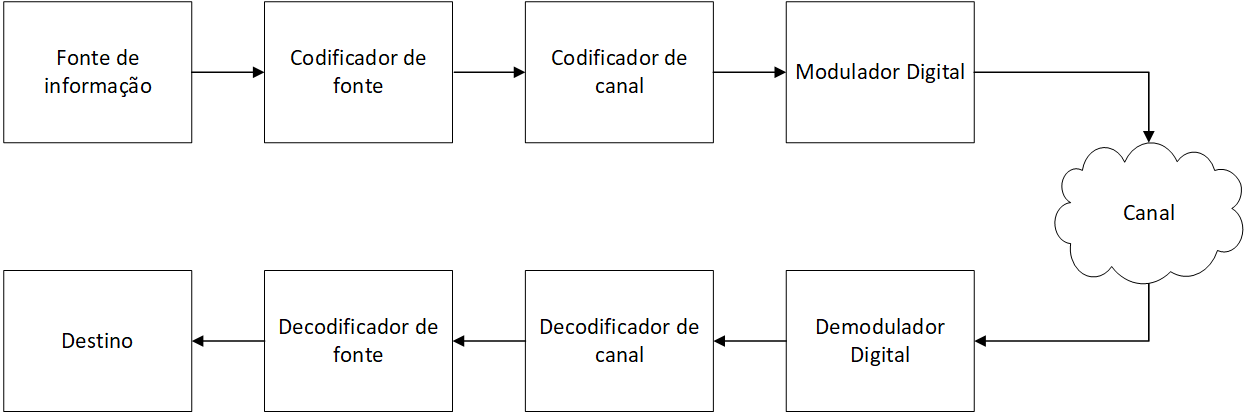
\includegraphics[scale=0.5]{./Figures/png/figura1.png}
\caption{Esquema em blocos de um sistema de comunicação digital.}
\label{fig:image_seq}
\end{center}
\end{figure}


Ao passar pelo canal, o sinal transmitido pode ser corrompido de forma aleatória por diversos mecanismos: adição de ruídos, atenuação, seletividade em frequência, deslocamento de fase, que são, em geral, dependentes do tempo. Estes diversos mecanismos podem comprometer a comunicação entre os dispositivos. 
 
Neste contexto, o uso de simulação é muito importante, pois a adoção de um padrão só é possível a partir do estudo, simulação e prototipação de um modelo definido. Para os sistemas de comunicação digitais, o desenvolvimento e teste de sistemas digitais, a comparação de desempenho de diferentes modelos de modulação, as restrições de custo nos testes e a necessidade de reproduzir condições ambientais onde o cenário possa ser repetido uma infinidade de vezes, dependem do suporte das simulações. 

\section{Justificativa e Motivações}

No desenvolvimento de modelos de comunicação, uma das técnicas mais empregadas consiste na simulação. Esta técnica, é considerada muito útil ao oferecer segurança na minimização de riscos e custos com diversos recursos e ações \cite{shannon1998introduction}.

A simulação é útil na resolução de problemas complexos que podem envolver situações determinísticas ou estocásticas. A simulação uma importante ferramenta de planejamento que procura emular, por meio de relações lógicas, o funcionamento de sistemas reais, a fim de observar seu comportamento sob diferentes cenários.

Os investimentos com modificações de produtos, processos, tecnologias e arranjos físicos são altos e arriscados. A simulação permite uma visualização mais detalhada do funcionamento da planta e ainda testes com cenários alternativos para indicar soluções a baixo custo, através de modelos computacionais.

Na área acadêmica a simulação possibilita estudar, em um ambiente virtual, o comportamento estático e dinâmico do modelo permitindo, dessa forma, projetar e prever a resposta do sistema sob investigação nas condições de trabalho que irão ocorrer no mundo real. A simulação, dessa forma, se apresenta, muitas vezes, como uma alternativa para reproduzir virtualmente experimentos que seriam muito onerosos.

Nesse contexto, a motivação deste TCC é: criar um software para simulação de um sistema de comunicação Digital utilizando faixa de frequência de 5 GHz. Para realizar este trabalho foi necessário a pesquisa de diversos pontos desta comunicação em artigos científicos e o aperfeiçoamento nas habilidades de programação em GNU Octave. 

\section{Objetivos}

Este trabalho propõe implementar um software que será utilizado para um ambiente de simulação de um sistema de comunicação digital usando o GNU Octave. O GNU Octave é uma Linguagem de Programação Científica que por ser um software livre que pode ser instalado gratuitamente em qualquer computador. Atualmente, está na versão 5.2.0. O GNU Octave pode ser executado em Windows, Linux e Mac OS \cite{octave}. 

Neste ambiente são abordados e comparados alguns parâmetros utilizados em um sistema de comunicação digital, tais como técnicas de modulação, nível de ruído na transmissão, entre outros. 

\section{Trabalhos Relacionados }

No trabalho de Aquino (2012) \cite{aquino2012modelo}, descreve a implementação de um sistema de comunicação digital usando o software Scilab, e levanta a possibilidade do software desenvolvido poder ser usado como ferramenta auxiliar em diversas disciplinas dos cursos técnicos em telecomunicações, tecnólogo em telemática, engenharia de telecomunicações. 

No estudo de Neto (2016) \cite{netoaprendendo}, cujo título é “APRENDENDO NA PRÁTICA: USO 
DO MATLAB® NO ESTUDO DA TAXA DE ERRO DE SÍMBOLO EM MODULAÇÕES M-ÁRIAS COM DETECÇÃO COERENTE”, nos apresenta a necessidade de meios de simulação em cursos de engenharia e demonstra a capacidade da integração lógica e prática por meio do auxílio da ferramenta Matlab® como escape para a ausência da prática. 

O trabalho de Cantu (2018) \cite{Cantur:2018:IFSC} propõe a implementação de um toolbox de funções de sincronismo de símbolo para a plataforma GNU Octave, este trabalho usuário possa migrar suas simulações que utilizam sincronizações da plataforma proprietária para a plataforma gratuita. 

Dentre várias pesquisas e protótipos desenvolvidos neste escopo, várias plataformas de simulação utilizadas e validadas como Scilab Aquino (2012) \cite{aquino2012modelo} e Matlab Yuting (2016) \cite{yuting2010simulation}, entretanto há uma carência de trabalhos utilizando GNU Octave. 

Neste trabalho, detectou-se a necessidade de ampliação dos estudos, através da implementação de um sistema de comunicação digital utilizando outra plataforma para simulação gratuita e de código livre, neste trabalho foi escolhido o GNU Octave. 


%\chapter{Fundamentos da compressão de imagens e vídeos}
%\thispagestyle{headings}
%%Capítulo 2 - Fundamentos de pompressão de imagens e vídeos%

\thispagestyle{fancy}

Neste capítulo abordam-se aspectos teóricos do processo de compressão de imagens e vídeos. Primeiramente, o conceito de redundância, presente em \textit{arrays} 2D, será abordado, fazendo-se a relação com a teoria da 
informação. Em seguida, é discutida uma possível classificação dos tipos de compressão com base na preservação do sinal original. Por fim, analisa-se o funcionamento dos padrões JPEG e MPEG-1.

\section{Redundância}
\label{redundancia}

O processo de compressão de dados consiste em reduzir a quantidade de bits necessária para representar uma determinada informação. Neste 
contexto, os conceitos de dados e informação são diferentes, pois os dados são os meios pelos quais as informações são transmitidas 
\cite{Gonzalez2006}.

Seguindo esta linha de raciocínio, uma informação pode ser representada de infinitas maneiras. Assim sendo, o questionamento a ser respondido quando se objetiva a compressão de dados é: qual representação forneceria o menor volume de dados sem que houvesse perda de informação?

A compressão é obtida através da eliminação dos dados redundantes presentes na representação de uma informação mantendo um dado critério de fidelidade. Em se tratando de 
\textit{arrays} bidimensionais, os principais tipos de redundância são \cite{Gonzalez2006}:

\begin{itemize}
 \item \textit{Redundância de codificação}: ocorre quando a quantidade de bits utilizada para representar os símbolos de uma determinada informação é superior à quantidade necessária. Este tipo de redundância é muito comum em métodos de codificação que trabalham com a atribuição de palavras-código de tamanho fixo.
 
 \item \textit{Redundância espacial e temporal}: devido à grande parte dos \textit{pixels} presentes em um \textit{array} 2D estarem espacialmente
 correlacionados, surge a redundância espacial. Já as sequências de vídeo estão sujeitas a mais outro tipo de redundância, a temporal, em que os pixels de quadros vizinhos encontram-se correlacionados devido à grande semelhança entre eles. Isso significa dizer que é possível alcançar maiores
taxas de compressao em vıdeos, do que em imagens estáticas.
 
 \item \textit{Redundância psicovisual}: é originada a partir das características do sistema visual humano. Sua resposta aos estímulos visuais é uma função
 não linear de grandezas físicas, como intensidade luminosa e cores. Neste contexto, pesquisas a respeito do funcionamento e comportamento do sistema visual humano são de grande importância para que possam ser gerados modelos matemáticos que representem características de tal sistema.
\end{itemize}



A quantificação do volume de dados redundantes presente em uma representação de imagem é necessária para que se possa avaliar a compressão obtida. Sendo assim, assumindo que $ b $ e $ b' $ são, respectivamente, o volume de dados presentes na representação real de uma imagem e o volume de dados
presentes em uma representação comprimida da mesma, a \textit{redundância relativa} $ R $ é dada por \cite{Gonzalez2006}
\begin{equation}
\label{eqR}
 R = 1-\frac{1}{c}
\end{equation}
em que $c$ é a \textit{taxa de compressão}, definida como sendo
\begin{equation}
\label{eqc}
 c=\frac{b}{b'}
\end{equation}

\section{Teoria da Informação}
\label{teoriadainformacao}

Durante a década de $ 40 $, no período da Segunda Guerra Mundial, o processo de troca de informações tornou-se fundamental. Dessa forma, surgiu a necessidade de estabelecer um limite mínimo de volume de bits necessário para a transmissão de uma determinada informação, a fim de otimizar a utilização do canal disponível.

Neste contexto, Claude Elwood Shannon ficou conhecido com o ``pai da teoria da informação'' ao propor com sucesso uma maneira de medir a incerteza sobre espaços desordenados \cite{shannon48}.

\subsection{Primeiro teorema de Shannon}
\label{shannonTheorem}
Através do teorema da codificação sem perda \cite{shannon48} pode-se provar que é possível representar a saída de um sistema sem memória com uma média $ H $ de unidades de informação por pixel,
\begin{equation}
\label{eqshannonTheorem}
\lim_{n \to \infty}
\left[\frac{L_{avg,n}}{n} \right]= H
\end{equation}
em que, $ L_{avg,n} $ é o número médio de códigos símbolo necessários para representar todos os grupos de $ n $ símbolos e $ H $ é a entropia.

\subsection{Entropia}
\label{entropia}

A entropia, equação \ref{eqentropia}, é uma medida utilizada em diversas áreas do conhecimento, como na química e física. Em se tratando de informações, a entropia representa o grau de incerteza de uma fonte.

Sendo (\textit{$a_{1}$,$a_{2}$,...,$a_{J}$}) o conjunto de símbolos (eventos) emitidos por uma determinanda fonte e $P(a_{1}), P(a_{2}), ..., P(a_{j})$ suas respectivas probabilidades de ocorrência, a informação contida em cada símbolo é
\begin{equation}
\label{eqentropia}
I(a_i) = \log_b{\frac{1}{P(a_{i})}}
\end{equation}
e a entropia é dada pela informação média dos símbolos.

\begin{equation}
\label{eqentropia}
H = -\sum_{j=1}^J P(a_{j})\log_b{P(a_{j})}
\end{equation}

No caso de imagens digitais, em que a unidade de representação é o \textit{bit}, tem-se que $ b = 2$ na equação \ref{eqentropia}.

\section{Métodos básicos de compressão}
\label{metodosdecompressao}

De maneira geral, existem dois tipos de compressão, com e sem perda, com as seguintes carcterísticas:

\begin{itemize}
\item Sem perda: objetiva comprimir o volume de dados necessários para representar uma dada informação sem que a mesma seja afetada. Para isso, códigos diferentes do código natural são atribuídos aos símbolos, a fim de reduzir a redundância de codificação. 

\item Com perda: objetiva alcançar um maior nível de compressão através da eliminação de elementos com base em critérios de qualidade exigidos pela aplicação de interesse.
\end{itemize}

\subsection{Métodos}
\label{metodos}

Existem vários métodos de codificação com e sem perda. Dentre eles, os mais utilizados são:

\begin{enumerate}
\item Sem perda:
\begin{itemize}
\item Huffman: a codificação de Huffman \cite{huf52} é um método de codificação de tamanho variável que consiste na atribuição de palavras código menores para símbolos mais frequentes e maiores para os símbolos menos frequentes.

O primeiro passo é rearranjar as probabilidades dos símbolos da fonte em ordem decrescente e fazer reduções sucessivas agrupando os símbolos de menor probabilidade de ocorrência, como na figura \ref{fig:huff_red}.

\begin{figure}[!ht]

\begin{minipage}{\textwidth}
    \begin{minipage}{.4\textwidth}
      \centering
      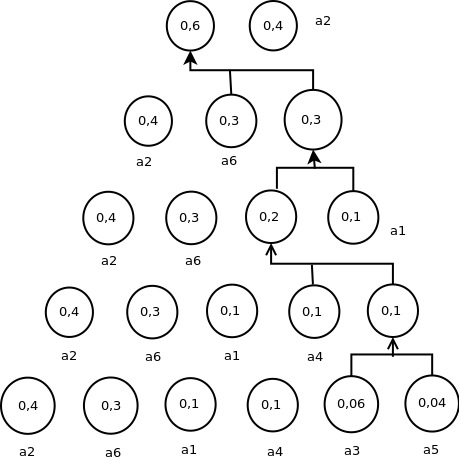
\includegraphics[width=.79\textwidth]{./Figures/png/huff_red.png}
      \caption{Reduções da fonte \cite{Gonzalez2006}.}
      \label{fig:huff_red}
    \end{minipage}
    \begin{minipage}{.56\textwidth}
    \center
      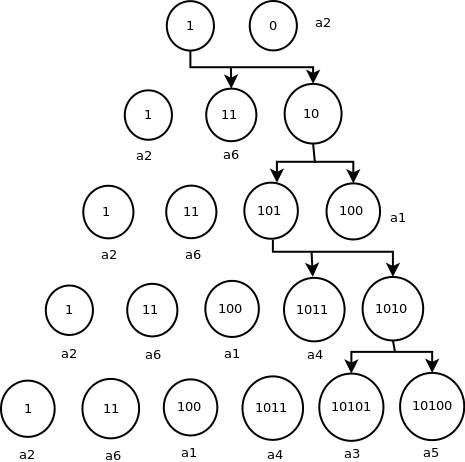
\includegraphics[width=.56\textwidth]{./Figures/png/huff_cod.png}
      \caption{Codificação da fonte reduzida \cite{Gonzalez2006}.}
      \label{fig:huff_cod}
    \end{minipage}
  \end{minipage}
\end{figure}

Por fim, deve-se codificar cada fonte reduzida seguindo o sentido inverso das reduções atribuindo $ 0 $ para as menores probabilidades e $ 1 $ para as maiores, ou vice-versa, como na figura \ref{fig:huff_cod}. Desta forma cada símbolo terá uma única palavra código cujo tamanho é inversamente proporcional a sua probabilidade de ocorrência.

\item Codificação aritmética: é um método de codificação de tamanho variável que trabalha de maneira bem diferente em relação à codificação de Huffman. Sua abordagem atribui faixas de valores, entre $ 0 $ e $ 1 $, para cada símbolo e por fim atribui palavras código aos intervalos \cite{Bhaskaran:1997:IVC:549617}.

Considerando o alfabeto $ s = (s1,s2,s3,s4) $, suponhamos que se queira codificar a mensagem $ s1s2s4$. Primeiramente calculam-se as probabilidades dos símbolos-fonte, as quais irão ocupar seguimentos proporcionais do intervalo $[0, 1]$. Depois deve-se fazer sucessivas divisões proporcionais dos símbolos dentro dos seguimentos, seguindo a ordem dos símbolos da mensagem, como na tabela \ref{arit_cod}.

\begin{table}[!ht]
\centering
\begin{tabular}{|c|c|c|c|c|c|}
\hline
$ s $ & $ p(s) $ & Faixa & $ s1$ & $ s1s2 $             & $ s1s2s4 $             \\ \hline 
s1            & 0,2           & {[}0,0; 0,2)         & {[}0,0; 0,04)  & {[}0,04;  0,048) & {[}0,072; 0,0736)   \\ \hline
s2            & 0,2           & {[}0,2; 0,4)         & {[}0,04; 0,08) & {[}0,048; 0,056) & {[}0,0736; 0,0752) \\ \hline
s3            & 0,4           & {[}0,4; 0,8)         & {[}0,08; 0,16) & {[}0,056; 0,072) & {[}0,0752; 0,0784) \\ \hline
s4            & 0,2           & {[}0,8; 1,0)         & {[}0,16; 0,2)  & {[}0,072; 0,08)  & {[}0,0784; 0,08)    \\ \hline
\end{tabular}
\caption{Exemplo de codificação aritmética.}
\label{arit_cod}
\end{table}

Por fim, escolhe-se um número dentro do intervalo atribuído para uma determinada mensagem que deverá representá-la	. No caso da mensagem $ s1s2s4 $,  foi atribuída a faixa $ [0,072; 0,08) $ e cada valor dentro da mesma poderá ser escolhido para representar esta mensagem.

\item Run-length: inicialmente produzida para a compressão para ser utilizada na tecnologia de FAX, cujas imagens são binárias. 

A codificação run-length é executada linha a linha começando com o valor inicial ($ 0 $ ou $ 1 $) seguido pelo número de repetições sucessivas. Quando houver a mudança de valor basta acrescentar o números de repetições sucessivas, pois sabe-se que o próximo valor é a negação do anterior.

\end{itemize}
\item Com perda:
\begin{itemize}
\item DPCM: Considerando que uma determinada amostra pode ser representada por 

\begin{equation}
\label{sinal_orig}
f(n) = \hat{f}(n) + e(n)
\end{equation}

em que $ \hat{f}(n) $ é uma aproximação da amostra original e $ e(n) $ é erro associado à mesma, o erro médio quadrático entre $ f $ e $ \hat{f} $  pode ser minimizado através de uma melhor aproximação do sinal original. 

Na codificação DPCM (Differential Pulse-Code Modulation), se $ e(n) \rightarrow 0 $, temos que a aproximação do sinal original pode ser representada por uma combinação linear descrita por

\begin{equation}
\label{sinal_pred}
\hat{f}(n) = \sum_{\substack{i=1}}^{m}\alpha_{i}f(n-i)
\end{equation}

em que os coeficientes são calculados através da minimização da expressão \ref{minimization}.

\begin{equation}
\label{minimization}
E \{ e(n)^{2} \} = E\left\{ \left[ f(n)- \sum_{\substack{i=1}}^{m}\alpha_{i}f(n-i)\right] ^{2} \right\}
\end{equation}

\item Codificação baseada em transformada de blocos: é uma técnica de compressão que consiste em dividir uma imagem em blocos não sobrepostos de tamanhos iguais (geralemente $ 8 \times 8 $). Uma transformada linear reversível, como a transformada de Fourier e a transformada cosseno, é utilizada para mapear estes blocos no domínio da frequência que por fim serão submetidos a um processo de quantização \cite{Gonzalez2006}.
\end{itemize}
\end{enumerate}

\section{Os padrões JPEG e MPEG-1}
\label{JPEGeMPEG}

O processo evolutivo da espécie humana deu-se de forma que a visão foi o sentido que mais se desenvolveu: cerca de $ 80-90\% $ dos neurônios estão relacionados com o processamento de informações visuais \cite{Young1991}. Dessa forma, não é de se surpreender que imagens e vídeos sejam cada vez mais explorados digitalmente.

Seguindo essa tendência, intensificaram-se as buscas por métodos capazes de otimizar a utilização da banda de transmissão sem que a informação seja prejudicada. Com base nisso surgiu a necessidade de padronização de métodos de compressão de imagens e vídeos, dando origem ao JPEG \cite{international1993ccitt}  e MPEG-1 \cite{telecommunication1993itu}, \cite{Bialkowski:2007:FVT:1290871.1290876}, \cite{1218189}.

\subsection{JPEG}
\label{jpeg}

Em meados da década de $ 80 $, a União Internacional de Telecomunicações (ITU, do inglês Iternational Telecommunication Union) concentrou seus esforços para a criação de um padrão de compressão de imagens estáticas. Desta forma deu-se a origem do JPEG.

Este padrão consiste em uma combinação de duas técnicas de compressão, com e sem perda (quantização e codificação de entropia). Como pode ser notado nas figuras \ref{fig:jpeg_enc} e \ref{fig:jpeg_dec}, o codificador e o decodificador, respectivamente, do \textit{JPEG baseline} \cite{Gonzalez2006} são destacados pela cor azul.

\begin{figure}[!ht]
  \begin{center}
    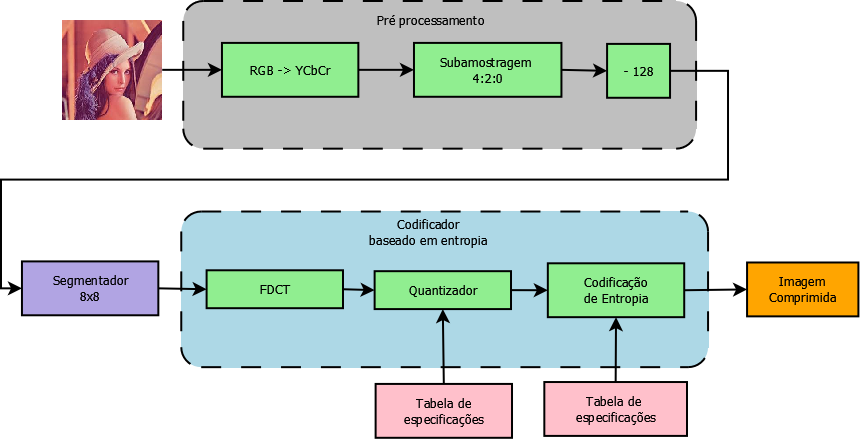
\includegraphics[scale=0.35]{./Figures/png/jpeg_encoder.png}
      \caption{Diagrama de blocos do codificador JPEG.}
      \label{fig:jpeg_enc}
  \end{center}
\end{figure}

\begin{figure}[!ht]
  \begin{center}
    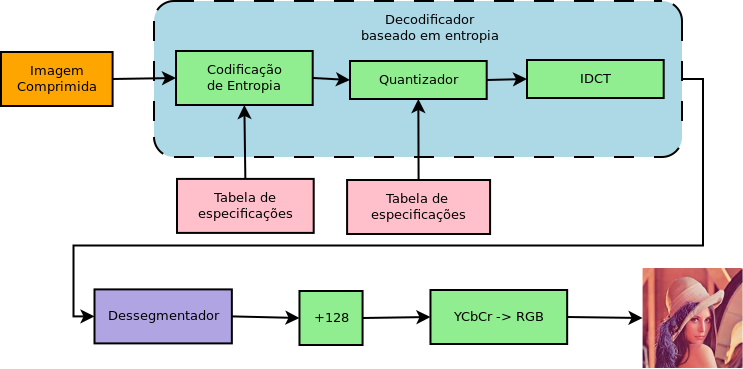
\includegraphics[scale=0.45]{./Figures/png/jpeg_decoder.png}
      \caption{Diagrama de blocos do decodificador JPEG.}
      \label{fig:jpeg_dec}
  \end{center}
\end{figure}

\subsubsection{JPEG baseline}
\label{JPEG_baseline}

Antes de detalhar o JPEG \textit{baseline} é importante citar que os canais de imagens RGB possuem um alto grau de correlação e carregam grande quantidade de informações espaciais, impossibilitando a eliminação de componentes da informação sem que a mesma seja fortemente afetada. Por isso o padrão JPEG trabalha com imagens YCbCr, que concentram a maior parte das informações espaciais no canal da luminância (Y) e as informações de cores nos canais restantes (Cb e Cr), possibilitando a eliminação de componentes de informação através da subamostragem da crominância \cite{Bhaskaran:1997:IVC:549617} no formato 4:2:0, detalhado no apêncide \ref{cro_diz}.

No sistema \textit{baseline} \cite{Gonzalez2006} o processo de compressão é composto por quatro passos sequenciais: segmentação, cálculo da transformada cosseno discreta, quantização e determinação dos códigos de tamanho variável para cada símbolo.

Inicialmente, a imagem é subdividida em blocos 8 $\times$ 8. Depois que os blocos são encontrados, seus valores são deslocados, subtraindo $ 2^{k-1} $ unidades, em que $ 2^{k} $ é o número máximo de níveis de intensidade. Então, aplica-se a transformada cosseno, onde $ p(x,y) $ é o valor do pixel na posição $ (x,y) $ e $ N $ é a ordem do bloco (oitava ordem) \cite{cabeen1998image},
\begin{equation}
\label{dct_eq}
D(i,j) = \frac{1}{\sqrt{2N}} C(i)C(j) \sum\limits_{x=0}^{N-1} \sum\limits_{y=0}^{N-1} p(x,y) \cos \left[ \frac{(2x+1)i \pi}{2N} \right] \cos \left[ \frac{(2y+1)j \pi}{2N} \right]
\end{equation}
\begin{equation}
C(u) = \begin{cases}
\frac{1}{\sqrt{2}} \quad \textrm{se } u = 0 \\
1 \quad \textrm{se } u > 0 \\ 
\end{cases} 
\end{equation}
 seguida pelo processo de quantização,
\begin{equation}
\label{eq_quant}
\hat{T}(u,v) = round \left(\frac{T(u,v)}{Z(u,v)}\right)
\end{equation}
em que $ \hat{T}(u,v) $ é o bloco quantizado (Fig.\ref{subimage_quant}), $ T(u,v) $ é o bloco transformado e $ Z(u,v) $ é a tabela de quantização padrão (Fig.\ref{quant_standard}) multiplicada por um fator de qualidade.

Através de experimentos subjetivos a respeito da percepção visual humana obteve-se a tabela de quantização padrão do JPEG. A utilização da mesma gera uma qualidade visual de $ 50\% $, que pode ser alterada multiplicando-a por um fator de qualidade: se a qualidade desejada for superior a $ 50 \% $ o fator usado deve ser $ (100-qualidade)/50 $, caso contrário o fator é $ 50/qualidade $.

\begin{figure}[!ht]\label{figuras_jpeg}
\subfigure[]{\label{quant_standard}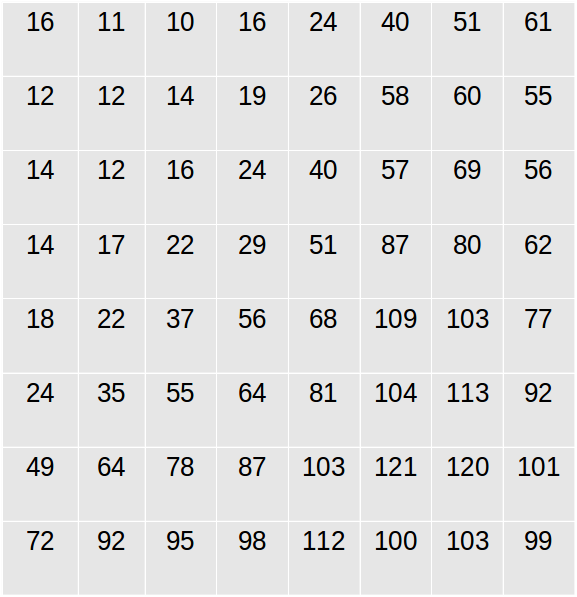
\includegraphics[width=.5\textwidth, height=.5\textwidth]{./Figures/png/tabela_padrao.png}}
\subfigure[]{\label{zigzag}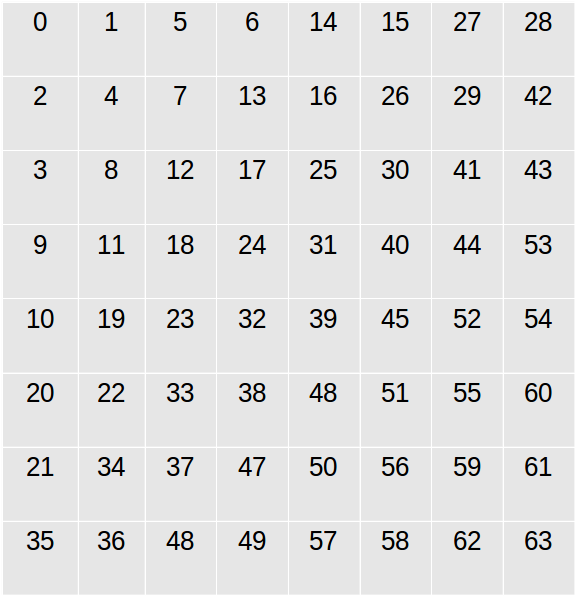
\includegraphics[width=.5\textwidth, height=.5\textwidth]{./Figures/png/zigzag.png}}
\subfigure[]{\label{subimage}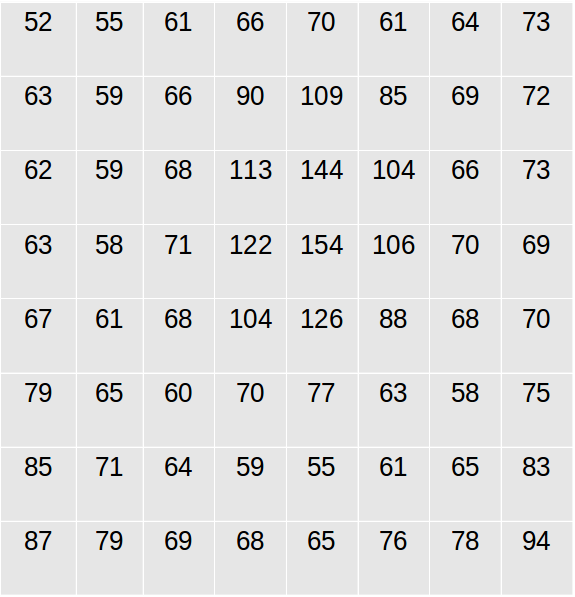
\includegraphics[width=.5\textwidth, height=.5\textwidth]{./Figures/png/subimage.png}}
\subfigure[]{\label{subimage_quant}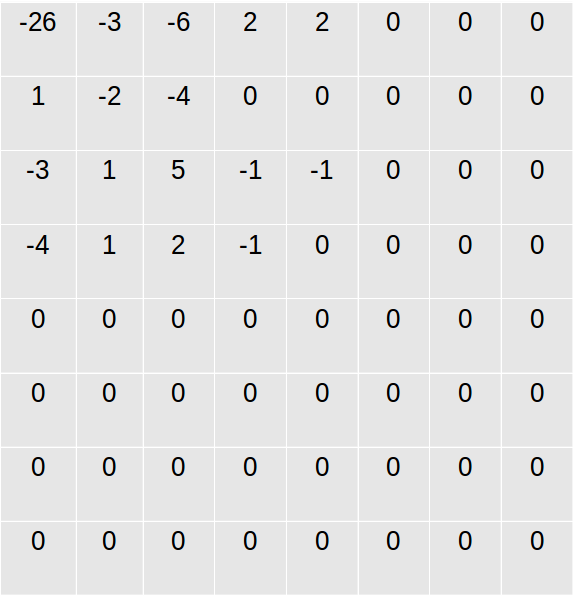
\includegraphics[width=.5\textwidth, height=.5\textwidth]{./Figures/png/subimage_quant.png}}
\caption{(a): Tabela de quantização padrão ($ 50 \% $); (b): Padrão zigzag; (c): Exemplo de subimagem; (d): Subimagem quantizada.}
\label{comp_visual}
\end{figure}

%\begin{table}[!ht]
%\begin{minipage}{.5\textwidth}
%\centering
%\begin{tabular}{|c|c|c|c|c|c|c|c|}
%\hline
%16 & 11 & 10 & 16 & 24  & 40  & 51  & 61  \\ \hline
%12 & 12 & 14 & 19 & 26  & 58  & 60  & 55  \\ \hline
%14 & 13 & 16 & 24 & 40  & 57  & 69  & 56  \\ \hline
%14 & 17 & 22 & 29 & 51  & 87  & 80  & 62  \\ \hline
%18 & 22 & 37 & 56 & 68  & 109 & 103 & 77  \\ \hline
%24 & 35 & 55 & 64 & 81  & 104 & 113 & 92  \\ \hline
%49 & 64 & 78 & 87 & 103 & 121 & 120 & 101 \\ \hline
%72 & 92 & 95 & 98 & 112 & 100 & 103 & 99  \\ \hline
%\end{tabular}
%\caption{Tabela de quantização padrão ($ 50 \% $).}
%\label{standard_table}
%\end{minipage} 
%\begin{minipage}{.5\textwidth}
%\centering
%\begin{tabular}{|c|c|c|c|c|c|c|c|}
%\hline
%0  & 1  & 5  & 6  & 14 & 15 & 27 & 28 \\ \hline
%2  & 4  & 7  & 13 & 16 & 26 & 29 & 42 \\ \hline
%3  & 8  & 12 & 17 & 25 & 30 & 41 & 43 \\ \hline
%9  & 11 & 18 & 24 & 31 & 40 & 44 & 53 \\ \hline
%10 & 19 & 23 & 32 & 39 & 45 & 52 & 54 \\ \hline
%20 & 22 & 33 & 38 & 46 & 51 & 55 & 60 \\ \hline
%21 & 34 & 37 & 47 & 50 & 56 & 59 & 61 \\ \hline
%35 & 36 & 48 & 49 & 57 & 58 & 62 & 63 \\ \hline
%\end{tabular}
%\caption{Padrão zigzag.}
%\label{zigzag}  
%\end{minipage}% 
%\vfill
%\begin{minipage}{.5\textwidth}
%\centering
%\begin{tabular}{|c|c|c|c|c|c|c|c|}
%\hline
%52 & 55 & 61 & 66 & 70  & 61  & 64  & 73  \\ \hline
%63 & 59 & 66 & 90 & 109  & 85  & 69  & 72  \\ \hline
%62 & 59 & 68 & 113 & 144  & 104  & 66  & 73  \\ \hline
%63 & 58 & 71 & 122 & 154  & 106  & 70 & 69  \\ \hline
%67 & 61 & 68 & 104 & 126  & 88 & 68 & 70  \\ \hline
%79 & 65 & 60 & 70 & 77 & 63 & 58 & 75 \\ \hline
%85 & 71 & 64 & 59 & 55 & 61 & 65 & 83 \\ \hline
%87 & 79 & 69 & 68 & 65 & 76 & 78 & 94  \\ \hline
%\end{tabular}
%\caption{Exemplo de subimagem.}
%\label{subimage_example}
%\end{minipage} 
%\begin{minipage}{.5\textwidth}
%\centering
%\begin{tabular}{|c|c|c|c|c|c|c|c|}
%\hline
%-26 & -3 & -6 & 2  & 2  & 0 & 0 & 0 \\ \hline
%1   & -2 & -4 & 0  & 0  & 0 & 0 & 0 \\ \hline
%-3  & 1  & 5  & -1 & -1 & 0 & 0 & 0 \\ \hline
%-4  & 1  & 2  & -1 & 0  & 0 & 0 & 0 \\ \hline
%0   & 0  & 0  & 0  & 0  & 0 & 0 & 0 \\ \hline
%0   & 0  & 0  & 0  & 0  & 0 & 0 & 0 \\ \hline
%0   & 0  & 0  & 0  & 0  & 0 & 0 & 0 \\ \hline
%0   & 0  & 0  & 0  & 0  & 0 & 0 & 0 \\ \hline
%\end{tabular}
%\caption{Subimagem da tabela \ref{subimage_example} quantizada.}
%\label{subimage_quantized}  
%\end{minipage}
%\end{table}

Por fim, os coeficientes dos blocos quantizados são reordenados no padrão zigzag (Tabela \ref{zigzag}), resultando em um vetor,

\begin{minipage}{1.\textwidth}
\centering
[-26 -3 1 -3 -2 -6 2 -4 1 -4 1 1 5 0 2 0 0 -1 2 0 0 0 0 0 -1 -1 EOB]
\end{minipage}
e codificados com base nas tabelas de Huffman pré definidas, as quais agrupam derivações dos métodos DPCM e run-length\footnote{A palavra código EOB significa que os coeficientes são iguais a $ 0 $ daquele ponto até o último coeficiente AC.}, como descrito no Apêndice \ref{ap_JPEG}.

O processo de decodificação é obtido através da simples inversão da ordem das operações.

\subsection{MPEG-1}
\label{mpeg}

O padrão H.261 \cite{ITU.1993} é um método versátil de compressão de vídeos com perda, pois pode ser aplicado a uma grande variedade de formatos de entrada. Porém, foi otimizado para aplicações que suportam taxas contínuas de transferência de bits de $ 1,5 $ Mbps.

Como mencionado na Seção \ref{redundancia}, os  vídeos estão sujeitos à redundância temporal devido à alta semelhança entre imagens vizinhas. Por isso, antes de falar do MPEG-1, é conveniente abordar o processo de estimação e compensação de movimentos baseado em blocos, a fim de eliminar a redundância temporal.

\subsubsection{Estimação e compensação de movimentos baseados em blocos}
\label{Est_Comp_Mov}

Objetivando-se reduzir a redundância temporal entre imagens consecutivas poder-se-ia pensar em armazenar apenas a diferença entre duas imagens, porém este processo pode ser otimizado através da utilização de macroblocos. Por isso pode-se dizer que este método é uma variação da codificação DPCM.

Macroblocos são compostos por 4 blocos $ n\times n $, na maioria das vezes 8$ \times $8. Na Figura \ref{fig:macrobloco} é representado um macrobloco subamostrado no padrão 4:2:0. Este padrão trabalha da seguinte forma:

\begin{figure}[!ht]
\begin{center}
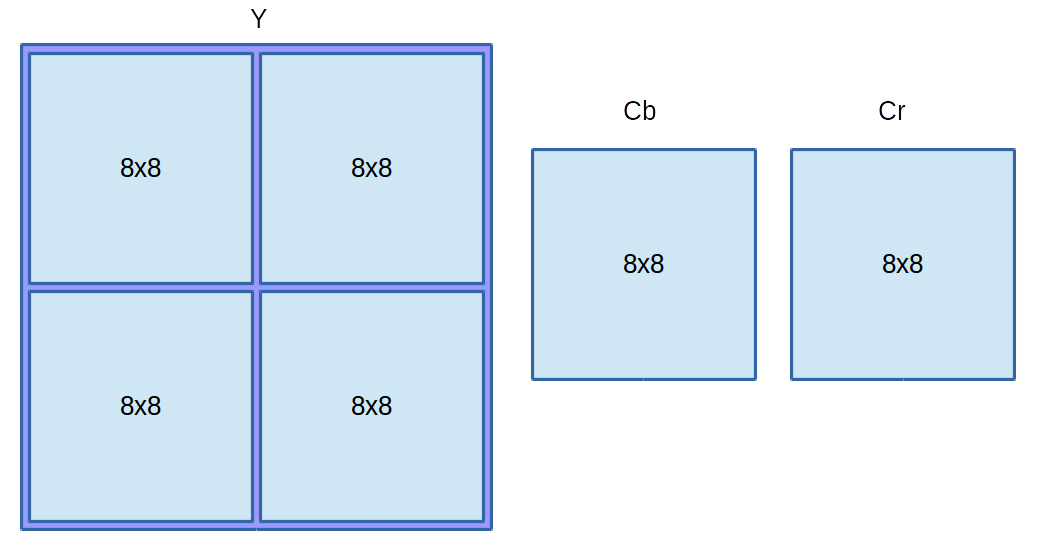
\includegraphics[scale=0.4]{./Figures/png/macrobloco.png}
\caption{Macrobloco dizimado no padrão 4:2:0.}
\label{fig:macrobloco}
\end{center}
\end{figure}

Utilizando macroblocos para a encontrar a diferença entre imagens consecutivas torna-se possível a minimização do erro médio absoluto (MAE, do inglês \textit{mean absolute error}) 
\begin{equation}
MAE(i,j) = \frac{1}{MN} \sum_{k=0}^{M-1} \sum_{l=0}^{N-1} |C(x+k,y+l)-R(x+i+k,y+j+l)
\end{equation}
da mesma, em que $C$ é um macrobloco da imagem de atual e $R$ o possível macrobloco correspondente na imagem de referência.

Inicialmente se considera uma imagem atual, em que se tem um macrobloco de dimensões 16$ \times $16 e uma imagem anterior com um macrobloco de mesmas dimensões com a menor diferença possível. Estes dois macroblocos possuem um deslocamento relativo designado por ``vetor de deslocamento'' e esta diferença é designada por ``erro de predição''. A este processo dá-se o nome de compensação de movimento para frente (Fig. \ref{fig:foreward_prediction}).

\begin{figure}[!ht]
\begin{center}
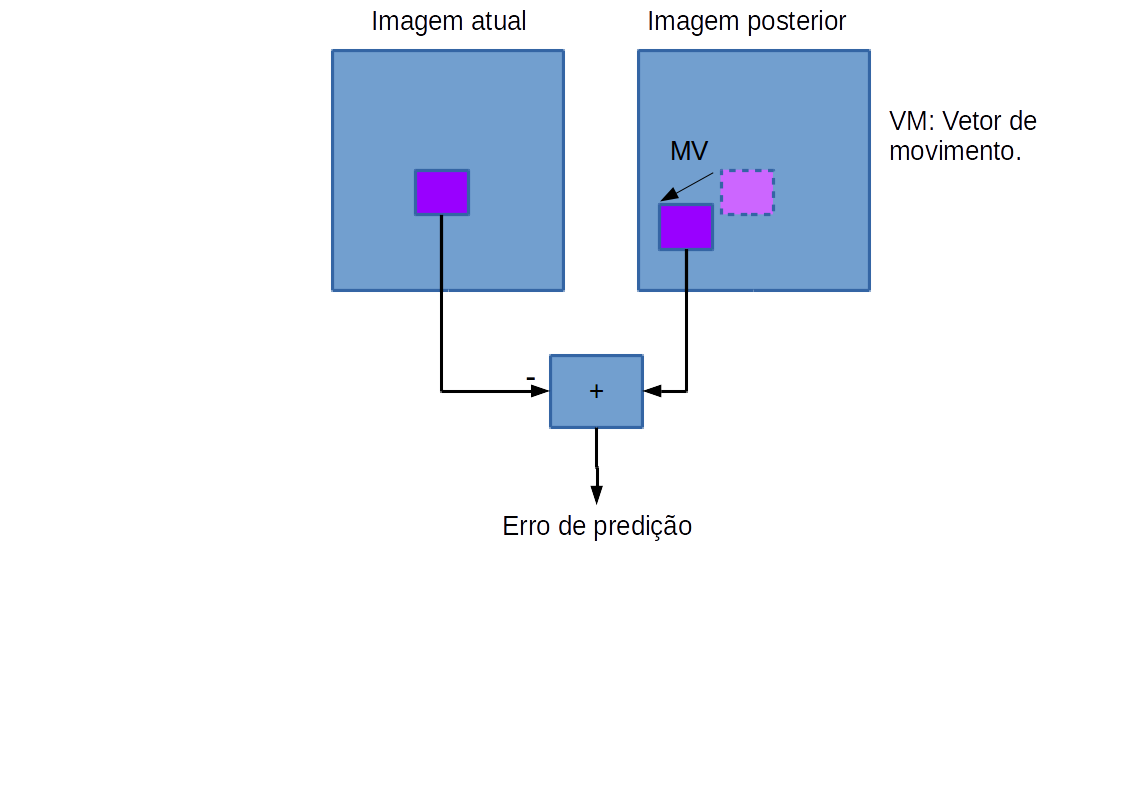
\includegraphics[scale=0.5]{./Figures/png/foreward_prediction.png}
\caption{Compensação de movimento pra frente.}
\label{fig:foreward_prediction}
\end{center}
\end{figure}

Também pode-se estender este raciocíno, tomando como base uma imagem atual, uma anterior e uma posterior a fim de obter a menor diferença possível. Este processo chama-se compensação de movimento bidirecional (Fig. \ref{fig:bidirectional_prediction}).

\begin{figure}[!ht]
\begin{center}
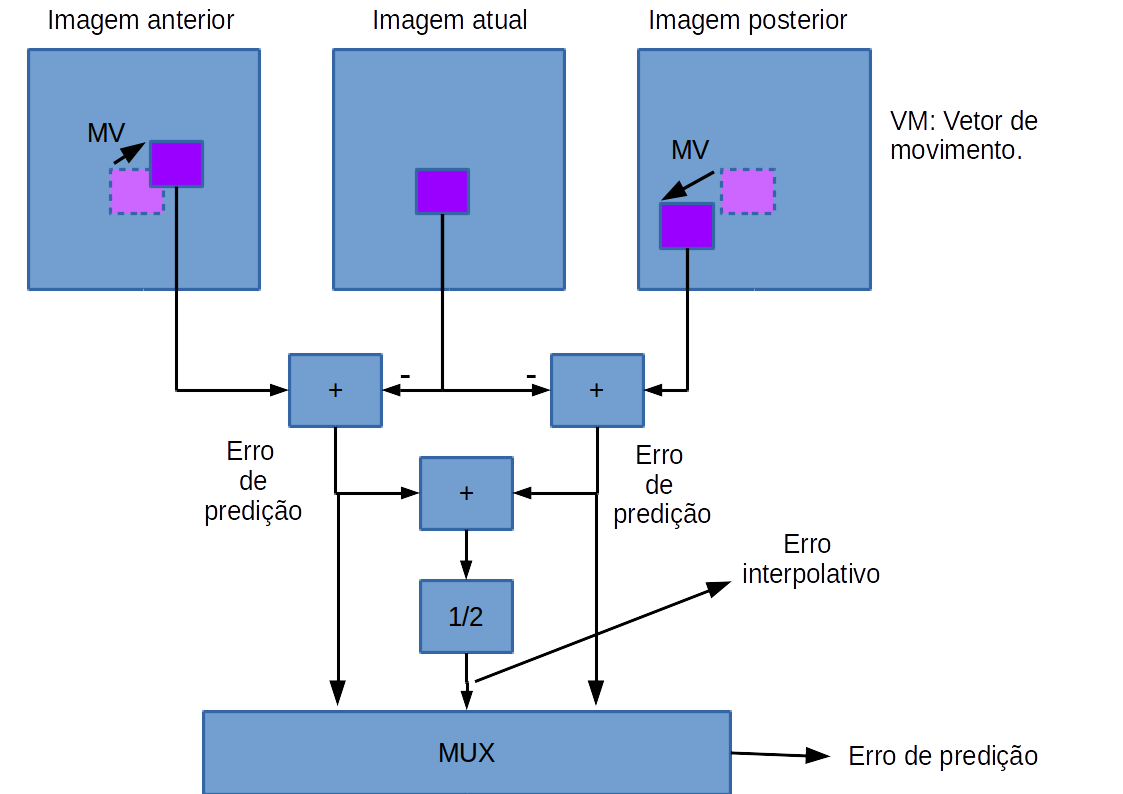
\includegraphics[scale=0.5]{./Figures/png/bidirectional_prediction.png}
\caption{Compensação de movimento bidirecional.}
\label{fig:bidirectional_prediction}
\end{center}
\end{figure}

A diferença fundamental entre os dois modelos de compensação de movimento é que o bidirecional trabalha com três erros de predição (para trás, para frente ou interpolativo) e não um, como na predição para frente. 

\subsubsection{Métodos de busca}

Há muitas formas de estimar os vetores de deslocamento dos macroblocos, algumas possibilitam uma maior precisão ao encontrar o melhor candidato, outras possibilitam uma maior velocidade na determinação do mesmo.

Dentre os métodos básicos, pode-se citar \cite{Bhaskaran:1997:IVC:549617}:
\begin{enumerate}
\item {\bf Busca completa:} é o método mais simples e garante que o melhor candidato seja encontrado, obtendo o menor valor possível do MAE.

Consiste na definição de uma área de busca de $ p $ pixels para os lados, para cima e para baixo a partir do canto superior esquerdo do macrobloco. Para cada um dos $ (2p+1)^2 $ pixels da área de busca serão formados os possíveis macroblocos a serem submetidos ao critério de minimização do MAE.

\item {\bf Busca unidimensional paralela hierárquica:} este método não garante o menor valor possível para o MAE, porém apresenta um ganho considerável em velocidade em comparação com método de busca completa.

Este algoritmo de busca é descrito da seguinte forma:
\begin{enumerate}
\item Para uma área de busca $ [-p,p] $, definida no método de busca completa, define-se $ S = 2^{\lfloor \log_{2}p \rfloor} $ e assumindo que a posição de origem $ (di,dj) $ do macrobloco seja $ (0,0) $.
\item Em paralelo, deve-se calcular:
\begin{itemize}
\item Para o eixo $ i $: encontrar dentre as três posições $ (di-S,dj) $, $ (di,dj) $ e $ (di+S,dj) $, qual delas gera o menor MAE. Por fim substituir $ di $ pela posição encontrada.
\item Para o eixo $ j $: encontrar dentre as três posições $ (di,dj-S) $, $ (di,dj) $ e $ (di,dj+S) $, qual delas gera o menor MAE. Por fim, substituir $ dj $ pela posição encontrada e $ S = \frac{S}{2}. $
\end{itemize}

O passo (b) deve ser repetido sucessivas vezes até que $ S=0 $. O vetor resultante $ (di,dj) $ será o vetor de deslocamento do macrobloco.
\end{enumerate}

\end{enumerate}

\subsubsection{Quantização}
\label{mpeg_quantization}

O processo de quantização utilizado no H.261 é similar ao utilizado no JPEG \textit{baseline}, diferindo apenas no fato de utilizar duas tabelas de quantização, para as codificações intra e inter imagens (Fig. \ref{tabelas_mpeg}).

\begin{figure}[!ht]\label{figuras_jpeg}
\subfigure[]{\label{fig:tabela_intra}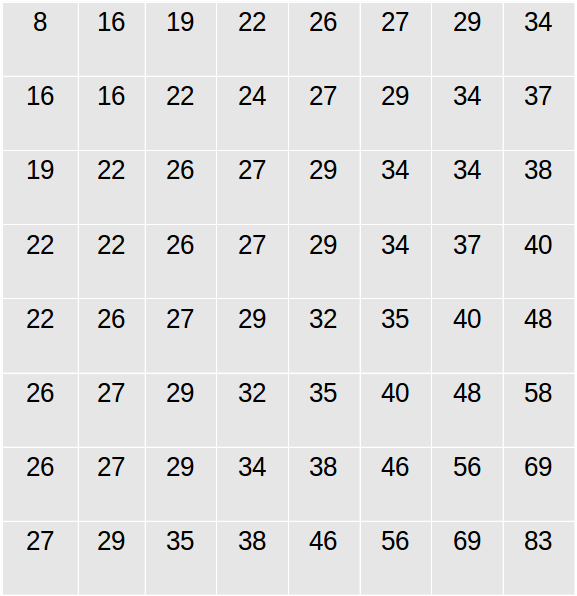
\includegraphics[width=.5\textwidth, height=.5\textwidth]{./Figures/png/tabela_intra.png}}
\subfigure[]{\label{fig:tabela_inter}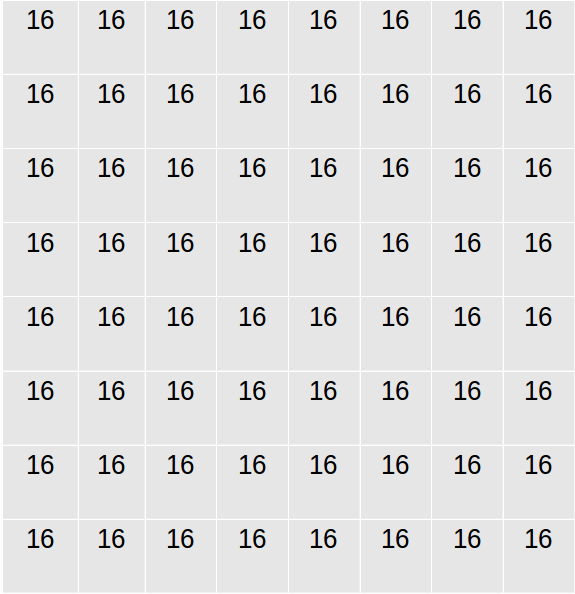
\includegraphics[width=.5\textwidth, height=.5\textwidth]{./Figures/png/tabela_inter.png}}
\caption{Tabelas intra (a) e inter (b).}
\label{tabelas_mpeg}
\end{figure}

%\begin{table}[!ht]
%\begin{minipage}{.5\textwidth}
%\centering
%\begin{tabular}{|c|c|c|c|c|c|c|c|}
%\hline
%8 & 16 & 19 & 22 & 26  & 27  & 29  & 34  \\ \hline
%16 & 16 & 22 & 24 & 27  & 29  & 34  & 37  \\ \hline
%19 & 22 & 26 & 27 & 29 & 34 & 34 & 38 \\ \hline
%22 & 22 & 26 & 27 & 29 & 34  & 37 & 40 \\ \hline
%22 & 26 & 27 & 29 & 32 & 35 & 40 & 48  \\ \hline
%26 & 27 & 29 & 32 & 35 & 40 & 48 & 58 \\ \hline
%26 & 27 & 29 & 34 & 38 & 46 & 56 & 69 \\ \hline
%27 & 29 & 35 & 38 & 46 & 56 & 69 & 83  \\ \hline
%\end{tabular}
%\caption{Tabela intra.}
%\label{standard_table_intra_mpeg}
%\end{minipage} 
%\begin{minipage}{.5\textwidth}
%\centering
%\begin{tabular}{|c|c|c|c|c|c|c|c|}
%\hline
%16 & 16 & 16 & 16 & 16 & 16 & 16 & 16 \\ \hline
%16 & 16 & 16 & 16 & 16 & 16 & 16 & 16 \\ \hline
%16 & 16 & 16 & 16 & 16 & 16 & 16 & 16 \\ \hline
%16 & 16 & 16 & 16 & 16 & 16 & 16 & 16 \\ \hline
%16 & 16 & 16 & 16 & 16 & 16 & 16 & 16 \\ \hline
%16 & 16 & 16 & 16 & 16 & 16 & 16 & 16 \\ \hline
%16 & 16 & 16 & 16 & 16 & 16 & 16 & 16 \\ \hline
%16 & 16 & 16 & 16 & 16 & 16 & 16 & 16 \\ \hline
%\end{tabular}
%\caption{Tabela inter.}
%\label{standard_table_inter_mpeg}  
%\end{minipage}
%\end{table}

É importante deixar claro que a necessidade de duas matrizes de quantização está relacionada com o fato de que, para as imagens preditas, as componentes de alta frequência não são necessariamente frequências espaciais, pois também podem ser provenientes do efeito de blocagem e das limitações o processo de compensação de movimento \cite{ghanbari2003standard}. Portanto, a padronização de uma tabela de quantização ponderada para as imagens inter codificadas seria uma tarefa muito complexa.

\subsubsection{Algoritmo}
\label{mpeg:algoritmo}

O padrão H.261 não reconhece entradas entrelaçadas, por isso utiliza-se a denominação de ``imagens'' e não ``frame''. Há três tipos de imagens que podem ser classificadas em dois métodos de compressão:

\begin{enumerate}
\item Intra imagem: as imagens I, como são conhecidades, são imagens que são codificadas de forma semelhante ao padrão JPEG. Neste tipo de codificação não há redução de redundância temporal, logo exige um volume de dados considerável para armazenamento.

\item Inter imagens: são imagens que passam pelo processo de compensação de movimentos em que as imagens de erro geradas são codificadas de forma semelhante ao JPEG.

Nesta classe se encaixam dois tipos de imagens, imagens P e B, que alcançam diferentes taxas de compressão:

\begin{itemize}
\item P (predita): basicamente a imagem é processada com base na imagem I ou P anterior, em que os vetores de deslocamento partem da imagem anterior para a imagem atual. Estas imagens alcançam maiores taxas de compressão quando comparadas com as imagens I.

\item B (bidirecionalmente predita): imagem processada com base na imagem I anterior e na imagem P posterior, ou vice sersa. A possibilidade de escolha entre dois erros de predição e o erro interpolativo possibilita que estas imagens alcancem taxas maiores de compressão quando comparadas com as imagens P.
\end{itemize}

\end{enumerate}

O processamento de imagens inter codificadas possui maior complexidade quando comparado com as imagens I, não apenas pela compensação de movimento mas também por casos especiais que ocorrem durante o processo de codificação, como:

\begin{enumerate}
\item A anulação de vetores de deslocamento ocorre em situações em que o erro de predição usando um vetor não nulo pode ser muito próximo do obtido através de um vetor nulo, pois neste caso a codificação dos vetores de deslocamento pode gerar a expansão do volume de dados necessários para a representação de um macrobloco.

Este é o procedimento padrão, a não ser que o erro de predição a partir de vetores não nulos seja no mínimo $ 1,1 $ vez menor que o obtido por vetores nulos.

\item Os macroblocos podem ser intra ou inter codificados. Pois há vezes em que a codificação intra é mais vantajosa do que a a inter.

\item Os macroblocos podem ou não ser codificados. A não codificação é utilizada quando todos os coeficientes quantizados da DCT são nulos, neste caso este macrobloco será uma cópia do presente na imagem de referência anterior.
\end{enumerate}

Para o codificador (Fig. \ref{fig:mpeg_enc}), inicialmente os canais Cb e Cr são subamostrados segundo o padrão 4:2:0 e define-se a ordem dos tipos de imagens dentro de um grupo de imagens (GOP, do inglês \textit{group of images}), de acordo com as necessidades. A mais comum é mostrada na figura \ref{fig:image_seq}.

\begin{figure}[!ht]
\begin{center}
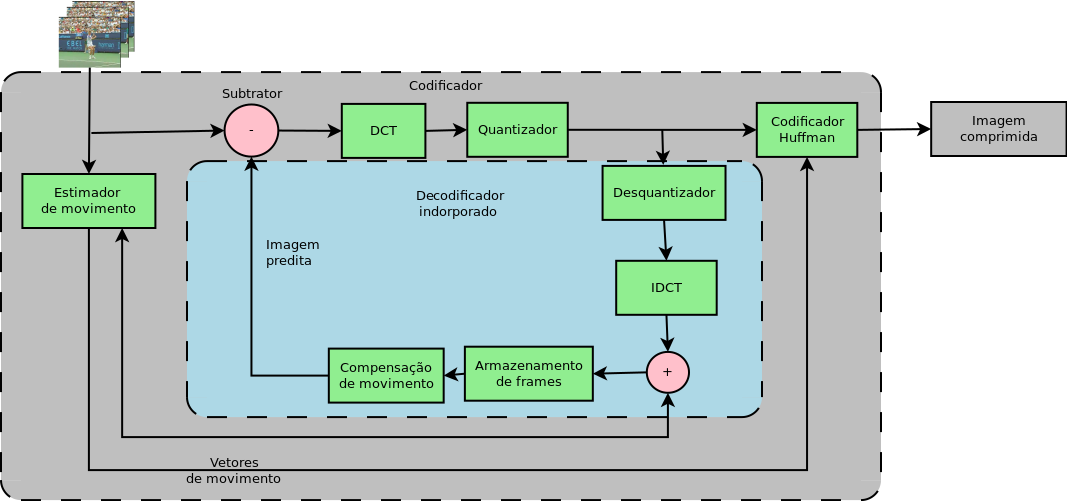
\includegraphics[scale=0.4]{./Figures/png/mpeg_encoder.png}
\caption{Diagrama em blocos do codificador MPEG.}
\label{fig:mpeg_enc}
\end{center}
\end{figure}

\begin{figure}[!ht]
\begin{center}
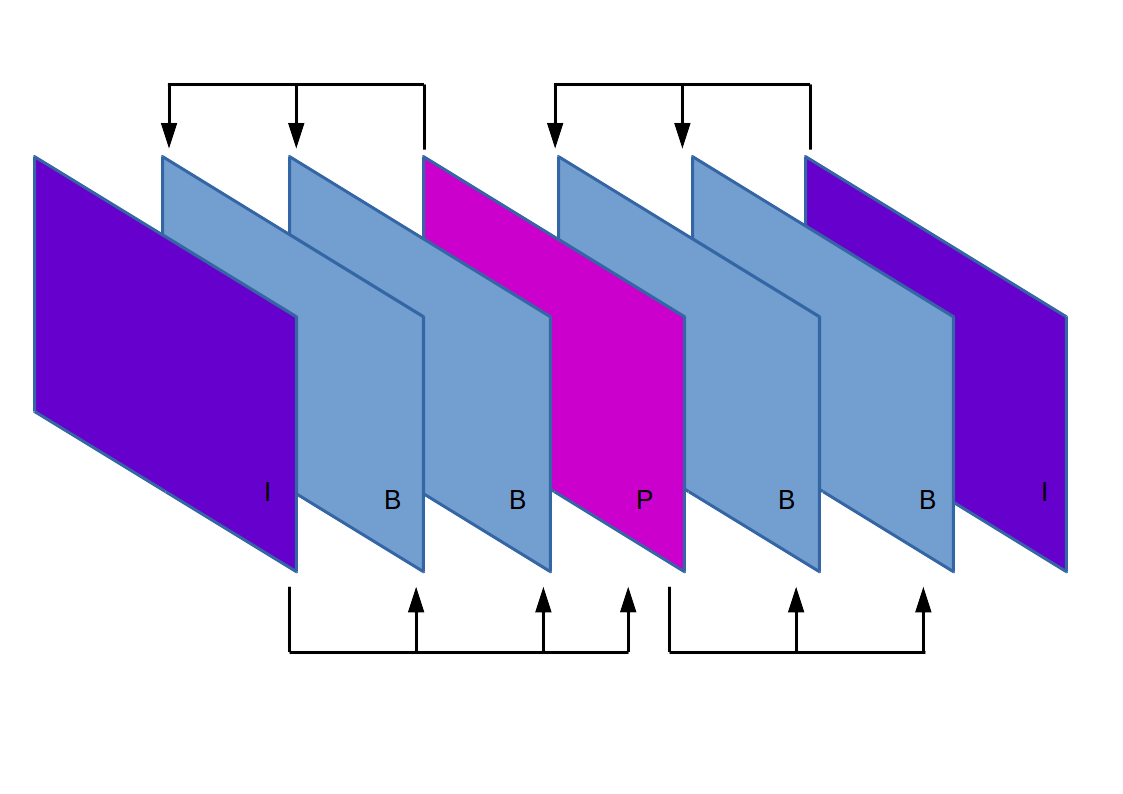
\includegraphics[scale=0.4]{./Figures/png/image_seq.png}
\caption{Sequência de imagens dentro de um GOP.}
\label{fig:image_seq}
\end{center}
\end{figure}

Depois que cada tipo de imagem foi processada, as imagens I, P e B são codificadas conforme descrito no padrão JPEG, porém as duas últimas utilizam a codificação de Huffman descrita no Apêndice \ref{ap_MPEG} para armazenar os vetores de deslocamento.

Para o decodificador (Fig. \ref{fig:mpeg_dec}), deve-se trabalhar por grupos de imagens, recuperando as imagens segundo o decodificador JPEG e recuperando as imagens ($P_1,P_2,P_3,...,P_n$) originais na ordem I, P, B, B, I, B e B para, se for necessário, realizar a compensação de movimento.

\begin{figure}[!ht]
\begin{center}
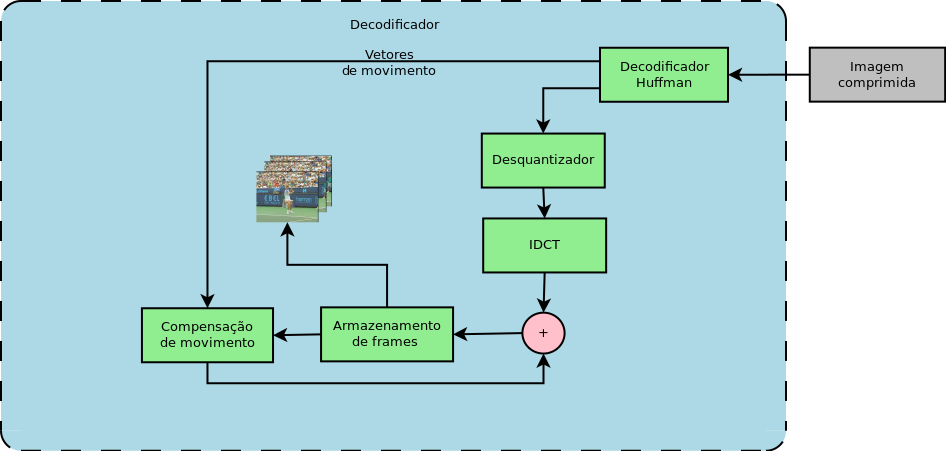
\includegraphics[scale=0.4]{./Figures/png/mpeg_decoder.png}
\caption{Diagrama em blocos do decodificador MPEG.}
\label{fig:mpeg_dec}
\end{center}
\end{figure}

%\chapter{Qualidade visual}
%\thispagestyle{headings}
%%Capítulo 3 - Os padrões JPEG e MPEG%

%Forward Error Correction (FEC) = Channel coding%
\thispagestyle{fancy}

``Uma imagem vale mais que mil palavras'', este ditado expressa a importância que os seres humanos dão às informações visuais. Não é de se espantar que existam grandes esforços voltados para pesquisas que objetivam encontrar métodos capazes de avaliar, bem como melhorar a qualidade visual de imagens e vídeos decodificados.

O conhecimento das cacterísticas do sistema visual humano (HVS, do inglês \textit{human visual system}) é fundamental para o desenvolvimento de metodologias eficazes no processo de avaliação e melhoria da qualidade visual de informações visuais. Embora o conhecimento do HVS seja muito limitado, há de se reconhecer que proporcionaram bons resultados, como em \cite{Li_humanvisual} e \cite{5941158}, em que são apresentados dois modelos de quantização adaptativa, um com base na percepção visual humana em determinadas frequências espaciais e temporais e outro que utiliza métricas de qualidade perceptual na fase de estimação de movimentos dos macroblocos, ambos alcançando bons resultados visuais em baixas taxas. Neste contexto, os processos de captura, exibição, armazenamento e transmissão deverão ser adaptados a fim de gerar representações mais exatas das imagens reais.


\section{Artefatos provenientes do processo de compressão}
\label{artefatos}

Na Seção \ref{JPEGeMPEG} foi mencionado que o JPEG e o MPEG-1 realizam uma quantização dos blocos tranformados, a fim de eliminar as redundâncias espacial e temporal. Em alguns sistemas este processo é o principal responsável pelo surgimento de distorções, apesar de não ser o único fator capaz de afetar a qualidade visual. Alguns dos tipos de artefatos mais comuns em sequências de vídeos são listados a seguir:

\begin{itemize}
\item Efeito de blocagem: ocorre devido à quantização independente de blocos, gerando descontinuidade nas fronteiras com blocos adjacentes.
\item Embaçamento: consequência da supressão das componentes de alta frequência durante o processo de quantização, manifestando-se através da perda da resolução espacial.
\item Vazamento de cores: devido aos processos de subamostragem de crominância seguido pela quantização, ocorre o vazamento de cores entre áreas de crominância muito diferentes.
\item Efeito de imagem base da DCT: ocorre quando uma única componente da DCT é dominante em um macro bloco, resultando na ênfase de uma imagem base da DCT.
\item Efeito ressonante: está relacionado com o fenômeno de Gibbs \cite{Gonzalez2006}, logo é mais evidente em áreas de grande contraste. Resultando da irregularidade de reconstrução das componentes de baixa frequência devido ao processo de quantização.
\item \textit{Aliasing}: ocorre quando a frequência de amostragem está abaixo da frequência de Nyquist \cite{Gonzalez2006}, tanto espacial quanto temporalmente.
\end{itemize}

\section{Avaliações subjetiva e objetiva}
\label{ava_subj_obj}

A melhor forma de conseguir avaliar a qualidade de informações visuais é através da opinião de observadores. A nota média de opiniões (\textit{mean opinion score}, MOS), avaliação subjetiva que necessita da opinião de um grupo de observadores, é a melhor forma de avaliar a qualidade de uma imagem se se pretende que essa avaliação seja de acordo com critérios de percepção humana. Porém, este método de avaliação perceptual demanda muito tempo para que se possa coletar um número considerável de opiniões.

Frequentemente o erro médio quadrático (\textit{mean square error}, MSE) é utilizado pelos métodos de avaliação de qualidade de imagens, devido a sua fácil implementação. No entanto, esses métodos apresentam baixo nível de correlação com as avaliações subjetivas, pois o MSE não leva em consideração características espaciais \cite{Wang2006}.

As pesquisas de avaliação objetiva de imagens buscam contornar os inconvenientes presentes na avaliação subjetiva, através de modelos matemáticos que simulam a percepção visual humana.

Há duas abordagens possíveis para o desenvolvimento de simuladores perceptuais: \textit{bottom-up} e \textit{top-down}.

Uma abordagem possível é estudar o funcionamento de cada elemento relevante para a percepção do sistema visual humano de forma a combiná-los em um sistema computacional. Esta abordagem é comumente conhecida como \textit{bottom-up}.

A outra abordagem possível é conhecida como \textit{top-down}, em que  o sistema é tido como uma caixa preta onde comportamentos hipotéticos são implemenados e ajustados. Os pontos atrativos desta abordagem são que o único conhecimento prévio necessário é a relação entre a entrada e a saída do sistema e a simplicidade de implementação.

\section{Classificação das métricas de avaliação de qualidade visual}
\label{metri_obj}

Segundo a disponibilidade de uma imagem de referência, para que uma métrica seja realmente útil para a avaliação de qualidade visual é necessário que ela seja capaz suprir as limitações do MSE. Logo, surgiram vários métodos que, a grosso modo, podem ser classificados em três categorias:

\begin{itemize}
\item Referência completa: há uma imagem de referência (considerada sem distorção) para avaliar uma imagem distorcida. Portanto, proporciona resultados mais precisos em relação a similaridade e fidelidade entre as duas imagens.
\item Sem referência: utilizada quando não é possível ter acesso a imagem referência, logo a avaliação da imagem distorcida deve ser feita as ``cegas'', o que faz disso uma tarefa difícil. Por isso esta categoria também é conhecida como de referência cega.
\item Referência reduzida: neste caso a imagem de referência não está completamente disponível e sim algumas características, que são embutidas no sistema que irá avaliar a imagen distorcida.
\end{itemize}

Outra classificação possível seria em relação à utilização das características do HVS. Neste caso, existem duas categorias:

\begin{itemize}
\item Perceptuais: são formulações matemáticas de certa complexidade inspiradas em
características fisiológicas e psicovisuais da visão que representam de forma automática a percepção humana perante uma representação de uma informação visual, com expressiva correlação com a real percepção humana.
\item Não perceptuais: não utilizam características do HVS nas suas formulações e têm como virtude a baixa
complexidade computacional. Porém, possuem baixa correlação com as avaliações subjetivas.
\end{itemize}

A seguir serão apresentadas métricas não perceptuais e perceptuais de especial interesse para este trabalho.

\subsection{Não perceptuais}
\label{nao_percep}

\subsubsection{Erro médio quadrático (Mean Square Error - MSE)}
\label{mse}

O MSE é uma métrica bastante utilizada que consiste no valor esperado do quadrado do erro,
\begin{equation}
MSE = E \left[ (y(i,j) - x(i,j))^2 \right]
\end{equation}
em que $ y $ é a imagem distorcida, $ x $ é a imagem de referência e $ (i,j) $ determina a posição dos pixels.
\subsubsection{Razão Sinal-Ruído (Signal-to-Noise Ratio - SNR)}
\label{snr}

Quantifica o quanto um sinal foi distorcido através do cálculo da razão entre a energia do sinal e a energia do erro associado à imagem distorcida.


A SNR é comumente medida em dB da seguinte forma,
\begin{equation}
SNR = 10\log_{10}{\frac{\sum_{i,j}[x(i,j)]^2}{\sum_{i,j}[x(i,j)-y(i,j)]^2}}
\end{equation}

\subsubsection{Razão Sinal-Ruído de Pico (Peak Signal-to-Noise Ratio - PSNR)}
\label{psnr}

É normalmente utilizada para medir a qualidade da reconstrução da imagem ou vídeo após uma compressão com perdas.

A PSNR é medida em dB da seguinte forma,
\begin{equation}
PSNR = 10\log_{10}{\frac{NK^2}{\sum_{i,j}[x(i,j)-y(i,j)]^2}}
\end{equation}
onde, $ N $ representa o número total de pixels da imagem e $ K $ representa o valor máximo que um pixel pode atingir. No caso de uma imagem de 8 bits/pixel o valor de $ K $  é 255.

\subsection{Perceptuais}
\label{perceptuais}



\subsubsection{Índice de Similaridade Estrutural (Structural Similarity Index - SSIM)}
\label{ssim}

O SSIM talvez seja a função de aproximação perceptual humana mais utilizada, devido a sua baixa complexidade de implementação em relação às demais e obter boas aproximações do HVS. Esta métrica avalia o quanto a estrutura da imagem de teste é diferente da estrutura da imagem de referência.

O SSIM é definido como
\begin{equation}
SSIM = \left[ l(x,y)^{\alpha}c(x,y)^{\beta}s(x,y)^{\gamma}
\right]
\end{equation}
em que $ \alpha > 0 $, $ \beta > 0 $ e $ \gamma > 0 $ são responsáveis pelo ajuste da importância relativa das
componentes $ l(x,y) $, $ c(x,y) $ e $ s(x,y) $ (correspondentes às componentes de luminância, contraste e estrutura, respectivamente) definidas como
\begin{equation}
l(x,y) = \frac{2 \mu_x \mu_y + c_1}{\mu_x^2 + \mu_y^2 + c_1}
\end{equation}
\begin{equation}
c(x,y) = \frac{2 \sigma_x \sigma_y + c_2}{\sigma_x^2 + \sigma_y^2 + c_2}
\end{equation}
\begin{equation}
s(x,y) = \frac{2 \sigma_{xy}+c_3}{\sigma_x \sigma_y + c_3}
\end{equation}
em que $ \mu_x $ e $ \sigma_x $ são a média e o desvio padrão da imagem $ x $; $ \mu_y $ e $ \sigma_y $ são a média e o desvio padrão da imagem $ y $; $ \sigma_{xy} $ é a covariância entre as imagens $ x $ e $ y $. Os termos $ c_1 $, $ c_2 $ e $ c_3 $ são inseridos com o objetivo de evitar instabilidades.

Esta métrica é aplicada localmente, deslocando, horizontalmente e verticalmente, uma janela de tamanho $B \times B$ sobre a imagem. Pode-se calcular a média do SSIM (MSSIM) para que se tenha uma índice de qualidade geral da imagem, em que $ M $ é o número de janelas e $SSIM_{j}$ é o SSIM associado à j-ésima janela.

\begin{equation}
MSSIM = \frac{1}{M}\sum_{j = 1}^{M}SSIM_{j}
\end{equation}

\section{Quantização inter-adaptativa baseada no HVS}
\label{QIBSVH}

A grosso modo, o sistema visual humano consegue captar pequenas variações de brilho em áreas relativamente grandes, mas não consegue captar com a mesma facilidade quando estas variações estão presentes em componentes de alta frequência \cite{Kelly1979}. Os sistemas de compressão obtêm vantagens desse fato ao quantizar fortemente as componentes de alta frequência e de maneira mas branda as componentes de baixa frequência. Como pode ser visto na figura \ref{fig:dct_comp_distr}, a DCT agrupa as componentes de baixa frequência no canto superior esquerdo e as de alta frequência no inferior direito do macrobloco transformado, possibilitando a produção de tabela de quantização apropriadas para o propósito mencionado.

\begin{figure}[!ht]
\begin{center}
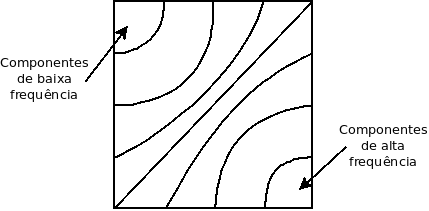
\includegraphics[scale=0.4]{./Figures/png/DCT_COMP.png}
\caption{Distribuição da frequência espacial no domínio da DCT.}
\label{fig:dct_comp_distr}
\end{center}
\end{figure}

O padrão H.261 \cite{telecommunication1993itu} utiliza o mesmo método de compressão para as imagens intra e inter codificadas. Atualmente vários métodos que levam em consideração as características do HVS têm sido propostos para melhorar a qualidade do vídeo reconstruído. 

Em \cite{Li_humanvisual}, um algoritmo de quantização inter adaptativo é proposto. Este algoritmo baseia-se no modelo apresentado por D. H. Kelly \cite{Kelly1979}, o qual afirma que o sistema visual humano é mais sensível às variações de contraste nas frequências espaciais intermediárias, ao passo que é menos sensível em frequências baixas e altas (Fig. \ref{fig:threshold_surface}). 
\begin{figure}[!ht]
\begin{center}
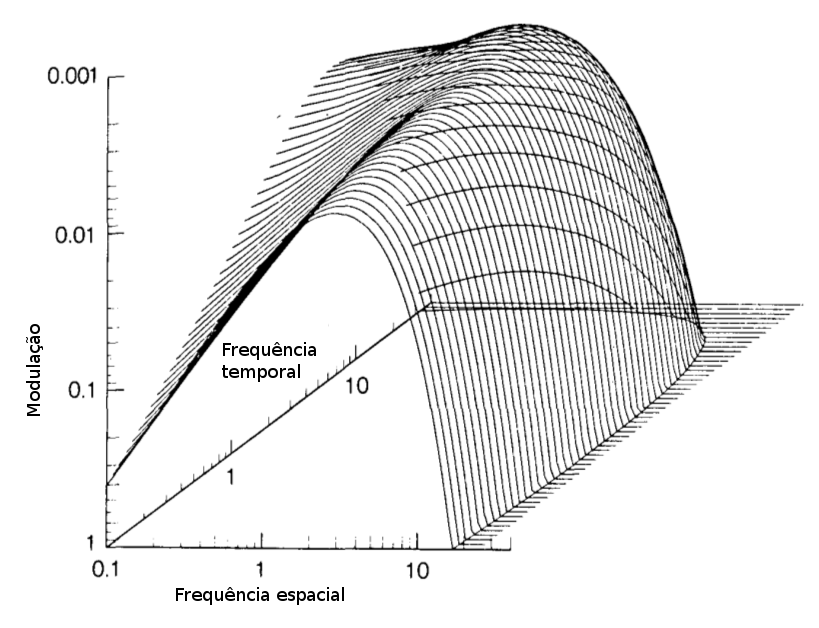
\includegraphics[scale=0.4]{./Figures/png/spatialtemporal_threshold.png}
\caption{Visão perspectiva da superfície de limiar espacial e temporal \cite{Kelly1979}. Cada curva representa a resposta à frequência espacial em uma frequência espacial fixa.}
\label{fig:threshold_surface}
\end{center}
\end{figure}
Tal algoritmo gera matrizes com base nas limitações do HVS em relação às respostas espaciais e temporais ao propor uma equação que representa a resposta do HVS à frequência temporal em função da velocidade e da frequência espacial do macrobloco,
\begin{equation}
G(\alpha,v) = \left[ 6.1 + 7.3 |\log(v/3)|^3 \right] v \alpha^2 \exp \left[ -2 \alpha (v+2)/45.9 \right]
\end{equation}
em que $ v $ velocidade do macrobloco, medida em graus por segundo, e $ \alpha $ é a frequência espacial medida em ciclos por segundo. Ambas são definidas por
\begin{equation}
v = (v_H^2 + v_T^2)^{1/2} 
\end{equation}
\begin{equation}
\quad \alpha_{ij} = \alpha_i + \alpha_j
\end{equation}
em que $ v_H $ e $ v_T $ são as componentes horizontal e vertical da velocidade do macrobloco e $ \alpha_i $ e $ \alpha_j $ são as componentes vertical e horizontal da frequência espacial. Ambas são definidas por
\begin{equation}
v_H = \frac{m_H}{w} \times f \quad \textrm{e} \quad v_T = \frac{m_T}{h} \times f
\end{equation}
\begin{equation}
\alpha_i = \frac{m_H}{m} \times \frac{w}{m} \times c_i \quad \textrm{e} \quad \alpha_j = \frac{m_T}{m} \times \frac{h}{m} \times c_j
\end{equation}
\begin{equation}
c_i = 0.5i \quad \textrm{e} \quad c_j = 0.5j \quad i,j = 1,0...7
\end{equation}
em que $ m_H $ e $ m_T $ são os valores absolutos das componentes do vetor de deslocamento do macrobloco\footnote{Logo, este método de quantização perceptual só é aplicado as imagens preditas (P, B), cuja qualidade depende diretamente do fator de qualidade das imagens I.}, $w$ e $h$ são as dimensões da imagem, e $m$ é o tamanho do macrobloco.

Com base no que foi mencionado, o modelo proposto em \cite{Li_humanvisual} objetiva melhorar a qualidade subjetiva do vídeo decodificado ao quantizar individualmente cada macrobloco respeitando as características do HVS,
\begin{equation}
\label{eq_qhvs}
Q_{HVS}(i,j) = (m_{H} + m_{T})/p \left( 1 - \frac{ G(\alpha_{ij},v) }{G_{max}} \right)
\end{equation}
em que $ Q_{HVS}(i,j) $ é uma componente do modelo de quantização visual, $ p $ é um parâmetro de ajuste e $ G_{max} $ é o valor máximo de $ G(\alpha, v) $.

Por fim, as matrizes de quantização a serem utilizadas são obtidas somando o modelo de quantização baseado no HVS a matriz de quantização plana.

\begin{equation}\label{perceptual_quant}
Q = Q_{flat} + Q_{HVS}
\end{equation}

Portanto, espera-se que a quantização adaptativa com base na sensibilidade do HVS a diferentes frequências espacial e temporal seja capaz de melhorar a qualidade perceptual dos vídeos decodificados, através da utilização da mesma no lugar da tabela de quantização inter imagens (Fig. \ref{fig:tabela_inter}).

%\chapter{Procedimento experimental e resultados}
%\thispagestyle{headings}
%%Capitulo 4 - análise e resultados%

\thispagestyle{fancy}

\section{Implementação do sistema}
\label{impl_sist}

Para a realização dos experimentos práticos apenas ferramentas livres foram utilizadas, em que um codec (codificador/decodificador) H.261 simplificado e o método de quantização perceptual inter-adaptativa (seção \ref{QIBSVH}) foram implementados em Python \cite{pythonbrasil} com auxílio da biblioteca OpenCV \cite{opencv}.

\section{Conjunto de teste}
\label{Conj_teste}

A análise do método de quantização perceptual \cite{Li_humanvisual} utilizado neste trabalho consiste em compará-lo com o utilizado no codificador H.261 padrão com diferentes condições. Para este procedimento, quatro vídeos  com diferentes características, obtidos em \cite{xiph_org}, serão utilizados (Tabela \ref{descr_videos}), de forma a analisar a compressão e a qualidade visual alcançada.

\begin{table}[!ht]
\centering
\begin{tabular}{|c|c|c|c|c|}
\hline
Vídeos       & \begin{tabular}[c]{@{}c@{}}Atividade\\ Temporal\end{tabular} & \begin{tabular}[c]{@{}c@{}}Duração\\ (seg) \end{tabular} & Resolução & FPS \\ \hline
Akiyo\_cif   & Baixa                                                        & 12            & 352 x 288 & 25  \\ \hline
Ice\_cif     & Baixa & 8             & 352 x 288 & 30  \\ \hline
Stefan\_cif  & Média & 3             & 352 x 288 & 25  \\ \hline
Foreman\_cif & Alta                                                         & 12            & 352 x 288 & 25  \\ \hline
\end{tabular}
\caption{Descrição dos vídeos.}
\label{descr_videos}
\end{table}

\section{Procedimento experimental}
\label{proc_experimental}

Os experimentos realizados tem dois objetivos: avaliar a viabilidade da utilização do método de quantização inter-adaptativa e avaliar a utilização de uma tabela plana em detrimento de uma ponderada para a quantização macroblocos preditos. 

Logo, o procedimento experimental é dividido em duas etapas, as quais foram submetidas a um processo de avaliação perceptual objetiva.

\begin{enumerate}
\item Para analisar em quais situações a quantização perceptual inter-adaptativa seria vantajosa, o codificador H.261 com e sem a mesma foi submetido a diferentes fatores de qualidade (0\%, 10\%, 20\%,..., 90\%, 100\%), de forma a gerar uma variação de taxa (kbps) em ambos os casos.

Neste trabalho utiliza-se o padrão H.261 e não o H.263, cujas magnitudes das componentes dos vetores de deslocamento são $ [-15; 15] $ e $ [-31,5; 31,5] $ respectivamente. Portanto, o modelo de quantização perceptual  utiliza deslocamento de busca de 15 pixels, a partir da origem, na horizontal e na vertical, $ p = 1 $, coeficientes de $ Q_{flat} $ iguais a 16 e as taxas (fps) utilizadas estão na Tabela \ref{descr_videos}.

\item Para estudar a viabilidade da utilização da tabela de quantização plana, a tabela ponderada utilizada nas imagens I será utilizada nas imagens P e B. O resultado proveniente desta configuração será comparado com os obtidos na análise anterior.
\end{enumerate}


\section{Resultados}
\label{resultados}

Analisando os resultados obtidos, na primeira fase do procedimento experimental, observa-se que para vídeos com pouco movimento, Figuras \ref{fig:mssim_akiyo} e \ref{fig:mssim_ice2}, o codec perceptual apresentou valores de MSSIM similares aos obtidos pelo codec convencional. Enquanto que para baixas taxas o codec perceptual apresentou um ganho de qualidade quando submetido a vídeos mais dinâmicos, Figuras \ref{fig:mssim_stefan} e \ref{fig:mssim_foreman}, confirmando a afirmação em \cite{Li_humanvisual} de que o método de quantização inter-adaptativa beneficia-se do aumento da atividade temporal.

A melhoria visual obtida pelo codec perceptutal deve-se à alocação diferenciada de bits para diferentes frequências espaciais de acordo com a influência que cada uma exerce sobre o HVS, resultando em uma redução do efeito de blocagem mais acentuado em baixas taxas, como pode ser confirmado através da figura \ref{comp_visual}.

É importante notar que o vídeo Akiyo\_cif apresentou um comportamento atípico para o gráfico de PSNR, ao ser comparado com o MSSIM, devido a este possuir maior correlação com a percepção visual humana, demonstrando ser o mais adequado para analisar a qualidade perceptual de informações visuais.

\begin{figure}[!ht]\label{MSSIN}
\subfigure[Akiyo.]{\label{fig:mssim_akiyo}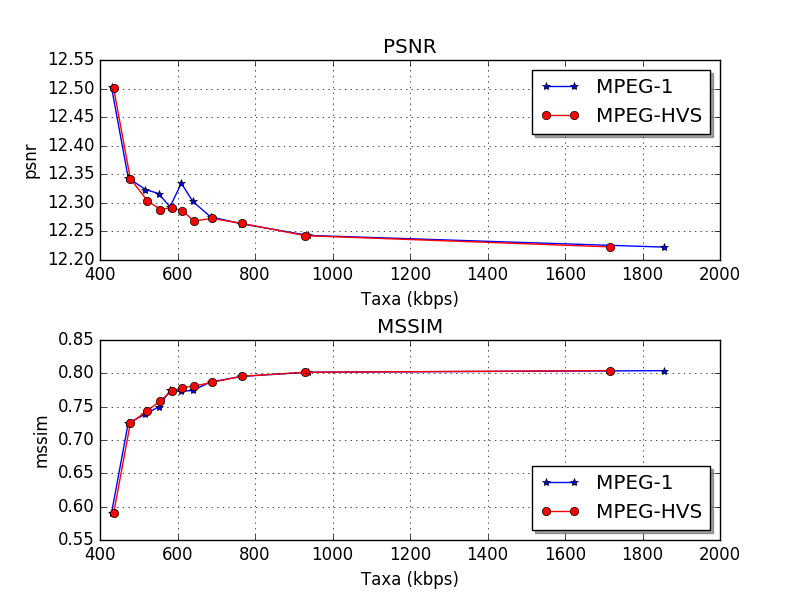
\includegraphics[width=.5\textwidth]{./Figures/png/akiyo_cif_vs_hvs.png}}
\subfigure[Ice.]{\label{fig:mssim_ice}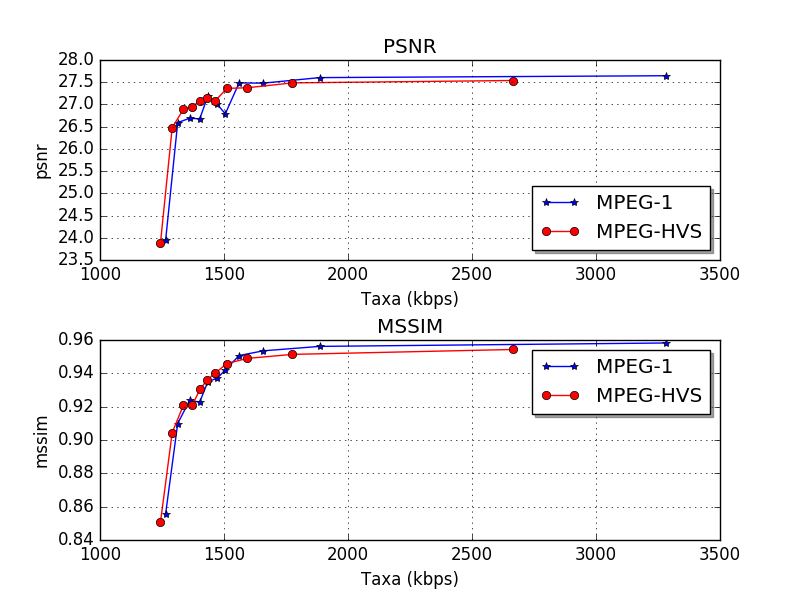
\includegraphics[width=.5\textwidth]{./Figures/png/ice_cif_vs_hvs.png}}
\subfigure[Stefan.]{\label{fig:mssim_stefan}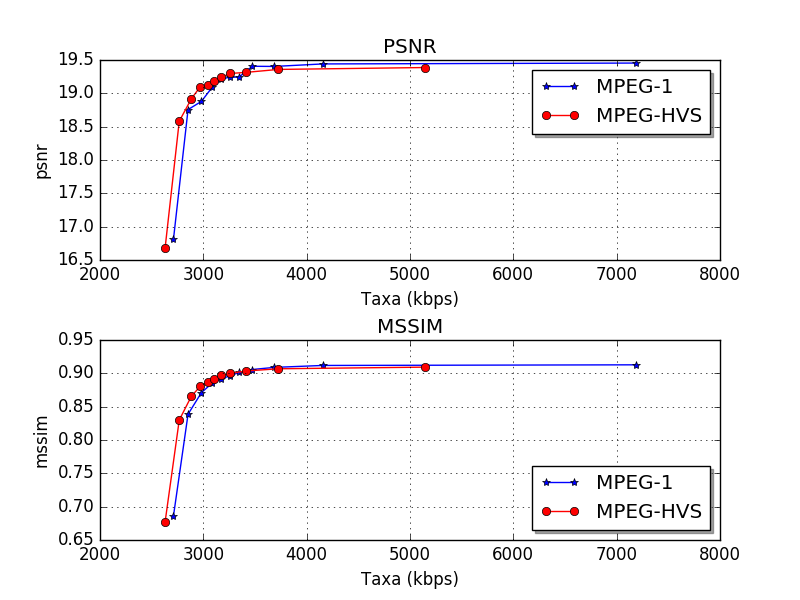
\includegraphics[width=.5\textwidth]{./Figures/png/stefan_cif_vs_hvs.png}}
\subfigure[Foreman.]{\label{fig:mssim_foreman}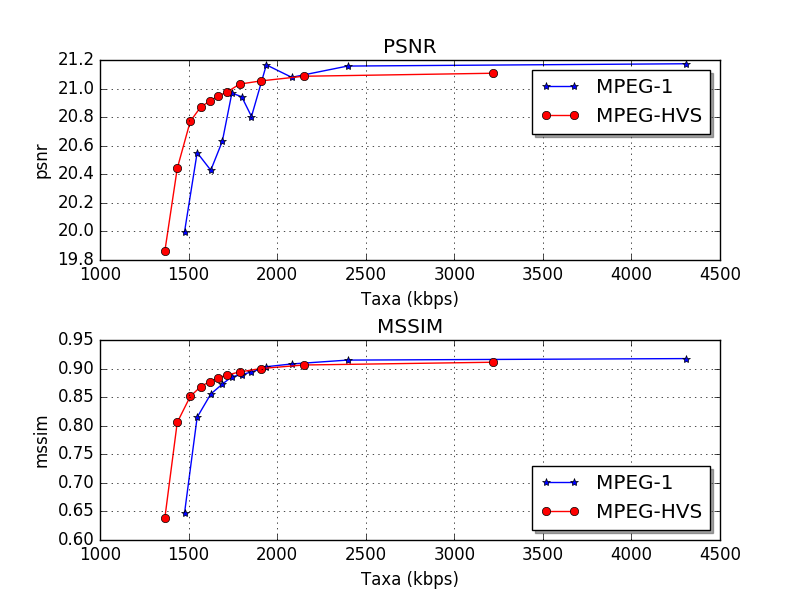
\includegraphics[width=.5\textwidth]{./Figures/png/foreman_cif_vs_hvs.png}}
\caption{Comparativo dos valores de MSSIM e PSNR pelos codecs padrão e perceptual.}
\end{figure}

\begin{figure}[!ht]\label{MSSIM}
\subfigure[]{\label{visu_standard}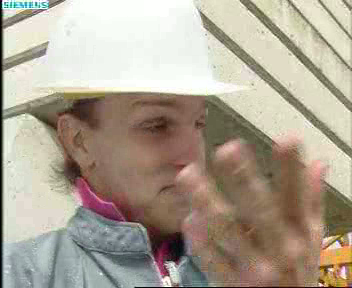
\includegraphics[width=.5\textwidth, height=.4\textwidth]{./Figures/png/foreman_155_1500.png}}
\subfigure[]{\label{visu_standard_cut}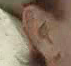
\includegraphics[width=.5\textwidth, height=.4\textwidth]{./Figures/png/foreman_155_1500_cut.png}}
\subfigure[]{\label{visu_perceptual}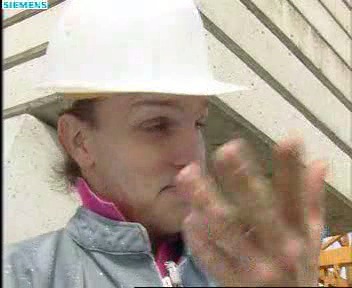
\includegraphics[width=.5\textwidth, height=.4\textwidth]{./Figures/png/foreman_hvs_155_1500.png}}
\subfigure[]{\label{visu_perceptual_cut}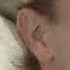
\includegraphics[width=.5\textwidth, height=.4\textwidth]{./Figures/png/foreman_hvs_155_1500_cut.png}}
\caption{Comparativo entre os codecs padrão, (a) e (b), e perceptual, (c) e (d).}
\label{comp_visual}
\end{figure}

\newpage

Utilizando a tabela ponderada (Fig. \ref{MSSIM_fase2}) de quantização na codificação das imagens P e B, os resultados obtidos são ainda mais interessantes. Diferentemente do que foi apontado em \cite{ghanbari2003standard}, pois essa adaptação gerou taxas (kbps) muito menores em comparação aos codificadores padrão e perceptual.

\begin{figure}[!ht]\label{MSSIM_fase2}
\subfigure[Akiyo.]{\label{fig:mssim_akiyo2}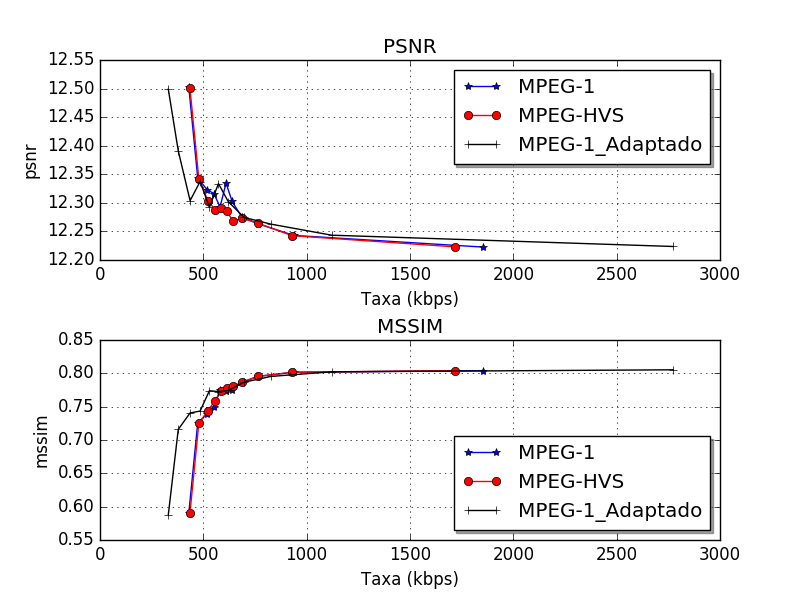
\includegraphics[width=.5\textwidth]{./Figures/png/akiyo_fase2.png}}
\subfigure[Ice.]{\label{fig:mssim_ice2}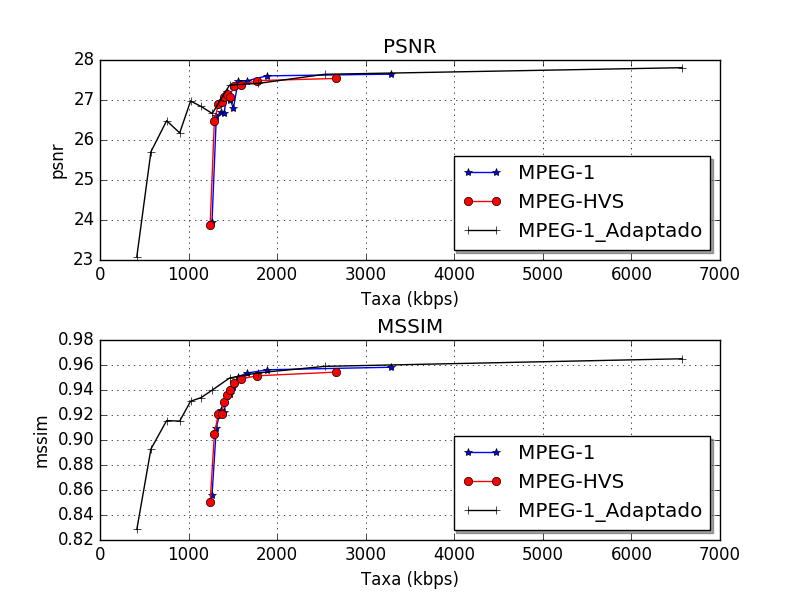
\includegraphics[width=.5\textwidth]{./Figures/png/ice_fase2.png}}
\subfigure[Stefan.]{\label{fig:mssim_stefan2}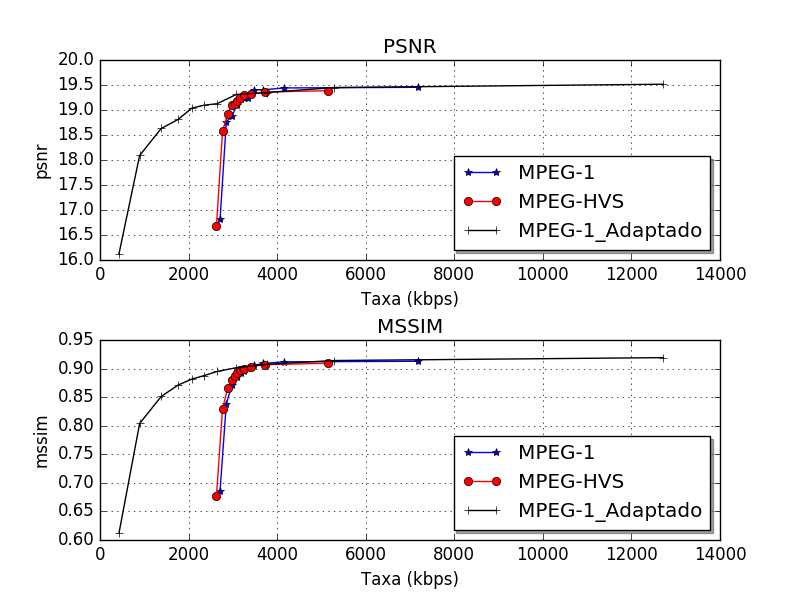
\includegraphics[width=.5\textwidth]{./Figures/png/stefan_fase2.png}}
\subfigure[Foreman.]{\label{fig:mssim_foreman2}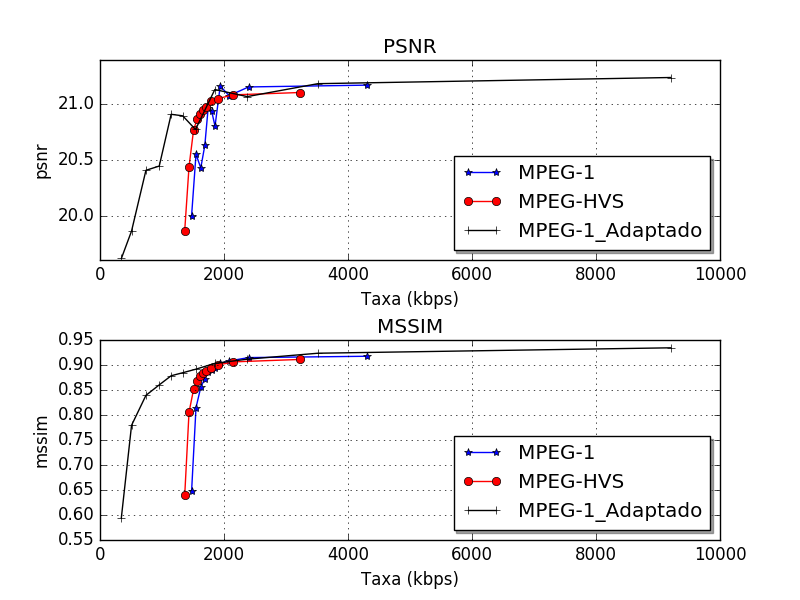
\includegraphics[width=.5\textwidth]{./Figures/png/foreman_fase2.png}}
\caption{Comparativo dos valores de MSSIM e PSNR pelos codecs padrão, padrão adaptado e perceptual.}
\end{figure}

Apesar dos resultados gerados pela utilização da tabela de quantização ponderada, em dentrimento da plana, terem se destacado como os mais eficienties, ainda não há, nesse trabalho, uma explicação plausível para esse comportamento.

%\chapter{Considerações finais}
%\thispagestyle{headings}
%%Capitulo 5 - Considerações finais%

\thispagestyle{fancy}

\section{Conclusões}

Neste trabalho foi apresentado um estudo de compressão de imagens e vídeos, através da análise teórica e implementações simplificadas dos codecs JPEG e MPEG-1. O aspecto perceptual dos vídeos decodificados também foi levado em consideração através da análise do método de quantização inter-adaptativa.

Apesar de necessário, o processo de compressão de informações visuais é responsável pelo surgimento de artefatos nas mesmas. Portanto, o desafio é encontrar um meio termo entre taxa de compressão e qualidade perceptual.

Através da análise desenvolvida neste trabalho pode-se concluir que a utilização do método de quantização inter-adaptativa gera resultados vantajosos para vídeos com alta atividade temporal, enquanto apresenta resultados similares ao codec padrão quando submetido a vídeos com baixa atividade temporal. Dessa forma, os resultados da avaliação objetiva obtidos neste trabalho então condizentes com os resultados subjetivos apresentados em \cite{Li_humanvisual}.

Portanto, a utilização do método de quantização inter-adaptativa é, se não vantajosa, no mínimo equivalente ao padrão H.261.

O mesmo não pode ser dito quando comparamos o codec H.261 utilizando apenas a tabela de quantização ponderada em relação aos codificadores analisados na primeira fase do experimento. Apesar da utilização de uma tabela plana para a quantização dos macroblocos inter codificados possuir embasamento teórico, \cite{ghanbari2003standard}, os resultados obtidos utilizando apenas a tabela ponderada foram os melhores alcançados neste trabalho, divergindo da literatura. No entanto, este resultado requer investigação mais ampla.

\section{Trabalhos futuros}

A próxima fase desta pesquisa tem como objetivos: obter o entendimento a respeito do funcionamento  de codecs mais atuais, como H.262, H.263, H.264 e H.265, de forma a entender as melhorias que foram ascrescentadas gradativamente; analisar de maneira mais profunda os resultados alcançados na segunda fase experimental e estudar outros métodos de melhoria de qualidade perceptual para armazenamento e vídeo conferência.

%\appendix
%\chapter{}
%\thispagestyle{headings}
%%Tabela de resultados de adições em um corpo GF($2^4$)

\thispagestyle{fancy}
\renewcommand{\thesubsection}{\Alph{section}}
\section{Tabelas de codificação para compressão JPEG}
\label{ap_JPEG}

Objetivando otimizar o processo de compressão JPEG, tabelas Huffman pré definidas são utilizadas para a codificação de entropia. Neste apêndice explica-se como utilizar estas tabelas.

Considerando que se deseja codificar um bloco transformado e quantizado,
\begin{minipage}{1.\textwidth}
\centering
[-26 -3 1 -3 -2 -6 2 -4 1 -4 1 1 5 0 2 0 0 -1 2 0 0 0 0 0 -1 -1 EOB]
\end{minipage}
devemos separar este processo em duas partes:
\begin{enumerate}
\item Codificação do coeficiente DC: supondo que o coeficiente DC do macrobloco imediatamente anterior é $ (-17) $, \footnote{Se for o primeiro macrobloco de uma linha utila-se o valor 0.} tem-se que, segundo a tabela \ref{Cat-coef-JPEG}, a diferença $ d = [-26-(-17)] $ ou $ d=-9 $ pertence à categoria $ k=4 $. Conforme a tabela \ref{Cod-DC}, o código base utilizado para a categoria 4 é 101 e seu tamanho total é de 7 bits, em que os $ k $ bits restantes devem ser os $ k $ bits menos significativos da diferença positiva $ d $ ou os $ k $ bits menos significativos da diferença negativa $ d $ menos $1$. Para a diferença $ d = -9$ os $k$ bits menos significativos são (0111)-1 ou 0110. Logo, a palavra código para o coeficiente DC em questão é 1010110.

\item Codificação do coeficiente AC: sua diferença em relação a codificação de coeficientes DC é que ela leva em consideração o número de zeros que antecedem os coeficientes AC não nulos. Logo o primeiro coeficiente AC não nulo $(-3)$ é codificado como 0100, pois segundo a tabela \ref{Cat-coef-JPEG} ele pertence à categoria 2 sem zeros antecedentes, dando origem ao código base 01, e os dois bits restantes são obtidos de maneira similar a utilizada na codificação de coeficientes DC. 
\end{enumerate}

\begin{table}[!ht]
\centering
\begin{tabular}{|c|c|c|}
\hline
Faixa                                                      & \begin{tabular}[c]{@{}c@{}}Categoria da\\ diferença DC\end{tabular} & \begin{tabular}[c]{@{}c@{}}Categoria\\ AC\end{tabular} \\ \hline
0                                                          & 0                                                                   & N/A                                                    \\ \hline
-1, 1                                                      & 1                                                                   & 1                                                      \\ \hline
-3, -2, 2, 3                                               & 2                                                                   & 2                                                      \\ \hline
-7,..., -4, 4,..., 7                                       & 3                                                                   & 3                                                      \\ \hline
-15,..., -8, 8,..., 15                                     & 4                                                                   & 4                                                      \\ \hline
-31,..., -16, 16,..., 31                                   & 5                                                                   & 5                                                      \\ \hline
-63,..., -32, 32,..., 63                                   & 6                                                                   & 6                                                      \\ \hline
-127,..., -64, 64,..., 127                                 & 7                                                                   & 7                                                      \\ \hline
-255,..., -128, 128,..., 255                               & 8                                                                   & 8                                                      \\ \hline
-511,..., -256, 256,..., 511                               & 9                                                                   & 9                                                      \\ \hline
-1023,..., -512, 5012,..., 1023                            & A                                                                   & A                                                      \\ \hline
-2047,..., -1024, 1024,..., 2047                           & B                                                                   & B                                                      \\ \hline
-4095,..., -2048, 2048,..., 4095                           & C                                                                   & C                                                      \\ \hline
-8191,..., -4096, 4096,..., 8191                           & D                                                                   & D                                                      \\ \hline
-16383,..., -8192, 8192,..., 16383                         & E                                                                   & E                                                      \\ \hline
\multicolumn{1}{|l|}{-32767,..., -16384, 16384,..., 32767} & F                                                                   & N/A                                                    \\ \hline
\end{tabular}
\caption{Categorias de coeficientes de codificação JPEG.}
\label{Cat-coef-JPEG}
\end{table}

\begin{table}[]
\centering
\begin{tabular}{|c|c|c|c|c|c|}
\hline
Categoria & \begin{tabular}[c]{@{}c@{}}Código\\ Base\end{tabular} & Tamanho & Categoria & \begin{tabular}[c]{@{}c@{}}Código \\ Base\end{tabular} & Tamanho \\ \hline
0         & 010                                                   & 3       & 6         & 1110                                                   & 10      \\ \hline
1         & 011                                                   & 4       & 7         & 11110                                                  & 12      \\ \hline
2         & 100                                                   & 5       & 8         & 111110                                                 & 14      \\ \hline
3         & 00                                                    & 5       & 9         & 1111110                                                & 16      \\ \hline
4         & 101                                                   & 7       & A         & 11111110                                               & 18      \\ \hline
5         & 110                                                   & 8       & B         & 111111110                                              & 20      \\ \hline
\end{tabular}
\caption{Códigos JPEG DC.}
\label{Cod-DC}
\end{table}

\begin{table}[!ht]
\centering
\begin{tabular}{|c|c|c|c|c|c|}
\hline
\begin{tabular}[c]{@{}c@{}}Zeros/\\ Categoria\end{tabular} & Código  base     & Tamanho & \begin{tabular}[c]{@{}c@{}}Zeros/\\ Categoria\end{tabular} & Código base      & Tamanho \\ \hline
0/0                                                        & 1010             & 4       & 8/1                                                        & 111111000        & 9       \\ \hline
0/1                                                        & 00               & 2       & 8/2                                                        & 111111111000000  & 15      \\ \hline
0/2                                                        & 01               & 2       & 8/3                                                        & 1111111110110110 & 16      \\ \hline
0/3                                                        & 100              & 3       & 8/4                                                        & 1111111110110111 & 16      \\ \hline
0/4                                                        & 1011             & 4       & 8/5                                                        & 1111111110111000 & 16      \\ \hline
0/5                                                        & 11010            & 5       & 8/6                                                        & 1111111110111001 & 16      \\ \hline
0/6                                                        & 1111000          & 7       & 8/7                                                        & 1111111110111010 & 16      \\ \hline
0/7                                                        & 11111000         & 8       & 8/8                                                        & 1111111110111011 & 16      \\ \hline
0/8                                                        & 1111110110       & 10      & 8/9                                                        & 1111111110111100 & 16      \\ \hline
0/9                                                        & 1111111110000010 & 16      & 8/A                                                        & 1111111110111101 & 16      \\ \hline
0/A                                                        & 1111111110000011 & 16      & 9/1                                                        & 111111001        & 9       \\ \hline
1/1                                                        & 1100             & 4       & 9/2                                                        & 1111111110111110 & 16      \\ \hline
1/2                                                        & 11011            & 5       & 9/3                                                        & 1111111110111111 & 16      \\ \hline
1/3                                                        & 1111001          & 7       & 9/4                                                        & 1111111111000000 & 16      \\ \hline
1/4                                                        & 111110110        & 9       & 9/5                                                        & 1111111111000001 & 16      \\ \hline
1/5                                                        & 11111110110      & 11      & 9/6                                                        & 1111111111000010 & 16      \\ \hline
1/6                                                        & 1111111110000100 & 16      & 9/7                                                        & 1111111111000011 & 16      \\ \hline
1/7                                                        & 1111111110000101 & 16      & 9/8                                                        & 1111111111000100 & 16      \\ \hline
1/8                                                        & 1111111110000110 & 16      & 9/9                                                        & 1111111111000101 & 16      \\ \hline
1/9                                                        & 1111111110000111 & 16      & 9/A                                                        & 1111111111000110 & 16      \\ \hline
1/A                                                        & 1111111110001000 & 16      & A/1                                                        & 111111010        & 9       \\ \hline
2/1                                                        & 11100            & 5       & A/2                                                        & 1111111111000111 & 16      \\ \hline
2/2                                                        & 11111001         & 8       & A/3                                                        & 1111111111001000 & 16      \\ \hline
2/3                                                        & 1111110111       & 10      & A/4                                                        & 1111111111001001 & 16      \\ \hline
2/4                                                        & 111111110100     & 12      & A/5                                                        & 1111111111001010 & 16      \\ \hline
2/5                                                        & 1111111110001001 & 16      & A/6                                                        & 1111111111001011 & 16      \\ \hline
2/6                                                        & 1111111110001010 & 16      & A/7                                                        & 1111111111001100 & 16      \\ \hline
2/7                                                        & 1111111110001011 & 16      & A/8                                                        & 1111111111001101 & 16      \\ \hline
\end{tabular}
\caption{Códigos JPEG AC.}
\label{Cod-AC1}
\end{table}


\begin{table}[!ht]
\centering
\begin{tabular}{|c|c|c|c|c|c|}
\hline
\begin{tabular}[c]{@{}c@{}}Zeros/\\ Categoria\end{tabular} & Código  base     & Tamanho & \begin{tabular}[c]{@{}c@{}}Zeros/\\ Categoria\end{tabular} & Código base      & Tamanho \\ \hline
2/8                                                        & 1111111110001100 & 16      & A/9                                                        & 1111111111001110 & 16      \\ \hline
2/9                                                        & 1111111110001101 & 16      & A/A                                                        & 1111111111001111 & 16      \\ \hline
2/A                                                        & 1111111110001110 & 16      & B/1                                                        & 1111111001       & 10      \\ \hline
3/1                                                        & 111010           & 6       & B/2                                                        & 1111111111010000 & 16      \\ \hline
3/2                                                        & 111110111        & 9       & B/3                                                        & 1111111111010001 & 16      \\ \hline
3/3                                                        & 111111110101     & 12      & B/4                                                        & 1111111111010010 & 16      \\ \hline
3/4                                                        & 1111111110001111 & 16      & B/5                                                        & 1111111111010011 & 16      \\ \hline
3/5                                                        & 1111111110010000 & 16      & B/6                                                        & 1111111111010100 & 16      \\ \hline
3/6                                                        & 1111111110010001 & 16      & B/7                                                        & 1111111111010101 & 16      \\ \hline
3/7                                                        & 1111111110010010 & 16      & B/8                                                        & 1111111111010110 & 16      \\ \hline
3/8                                                        & 1111111110010011 & 16      & B/9                                                        & 1111111111010111 & 16      \\ \hline
3/9                                                        & 1111111110010100 & 16      & B/A                                                        & 1111111111011000 & 16      \\ \hline
3/A                                                        & 1111111110010101 & 16      & C/1                                                        & 1111111010       & 10      \\ \hline
4/1                                                        & 111011           & 6       & C/2                                                        & 1111111111011001 & 16      \\ \hline
4/2                                                        & 1111111000       & 10      & C/3                                                        & 1111111111011010 & 16      \\ \hline
4/3                                                        & 1111111110010110 & 16      & C/4                                                        & 1111111111011011 & 16      \\ \hline
4/4                                                        & 1111111110010111 & 16      & C/5                                                        & 1111111111011100 & 16      \\ \hline
4/5                                                        & 1111111110011000 & 16      & C/6                                                        & 1111111111011101 & 16      \\ \hline
4/6                                                        & 1111111110011001 & 16      & C/7                                                        & 1111111111011110 & 16      \\ \hline
4/7                                                        & 1111111110011010 & 16      & C/8                                                        & 1111111111011111 & 16      \\ \hline
4/8                                                        & 1111111110011011 & 16      & C/9                                                        & 1111111111100000 & 16      \\ \hline
4/9                                                        & 1111111110011100 & 16      & C/A                                                        & 1111111111100001 & 16      \\ \hline
4/A                                                        & 1111111110011101 & 16      & D/1                                                        & 11111111000      & 10      \\ \hline
5/1                                                        & 1111010          & 7       & D/2                                                        & 1111111111100010 & 16      \\ \hline
5/2                                                        & 11111110111      & 11      & D/3                                                        & 1111111111100011 & 16      \\ \hline
5/3                                                        & 1111111110011110 & 16      & D/4                                                        & 1111111111100100 & 16      \\ \hline
5/4                                                        & 1111111110011111 & 16      & D/5                                                        & 1111111111100101 & 16      \\ \hline
5/5                                                        & 1111111110100000 & 16      & D/6                                                        & 1111111111100110 & 16      \\ \hline
5/6                                                        & 1111111110100001 & 16      & D/7                                                        & 1111111111100111 & 16      \\ \hline
\end{tabular}
\caption{Códigos JPEG AC (continuação.)}
\label{Cod-AC2}
\end{table}

\begin{table}[!ht]
\centering
\begin{tabular}{|c|c|c|c|c|c|}
\hline
\begin{tabular}[c]{@{}c@{}}Zeros/\\ Categoria\end{tabular} & Código  base     & Tamanho & \begin{tabular}[c]{@{}c@{}}Zeros/\\ Categoria\end{tabular} & Código base      & Tamanho \\ \hline
5/7                                                        & 1111111110100010 & 16      & D/8                                                        & 1111111111101000 & 16      \\ \hline
5/8                                                        & 1111111110100011 & 16      & D/9                                                        & 1111111111101001 & 16      \\ \hline
5/9                                                        & 1111111110100100 & 16      & D/A                                                        & 1111111111101010 & 16      \\ \hline
5/A                                                        & 1111111110100101 & 16      & E/1                                                        & 1111111111101011 & 11      \\ \hline
6/1                                                        & 1111011          & 7       & E/2                                                        & 1111111111101100 & 16      \\ \hline
6/2                                                        & 111111110110     & 12      & E/3                                                        & 1111111111101101 & 16      \\ \hline
6/3                                                        & 1111111110100110 & 16      & E/4                                                        & 1111111111101110 & 16      \\ \hline
6/4                                                        & 1111111110100111 & 16      & E/5                                                        & 1111111111101111 & 16      \\ \hline
6/5                                                        & 1111111110101000 & 16      & E/6                                                        & 1111111111110000 & 16      \\ \hline
6/6                                                        & 1111111110101001 & 16      & E/7                                                        & 1111111111110001 & 16      \\ \hline
6/7                                                        & 1111111110101010 & 16      & E/8                                                        & 1111111111110010 & 16      \\ \hline
6/8                                                        & 1111111110101011 & 16      & E/9                                                        & 1111111111110011 & 16      \\ \hline
6/9                                                        & 1111111110101100 & 16      & E/A                                                        & 1111111111110100 & 16      \\ \hline
6/A                                                        & 1111111110101101 & 16      & F/0                                                        & 11111111001      & 11      \\ \hline
7/1                                                        & 11111010         & 8       & F/1                                                        & 1111111111110101 & 16      \\ \hline
7/2                                                        & 111111110111     & 12      & F/2                                                        & 1111111111110110 & 16      \\ \hline
7/3                                                        & 1111111110101110 & 16      & F/3                                                        & 1111111111110111 & 16      \\ \hline
7/4                                                        & 1111111110101111 & 16      & F/4                                                        & 1111111111111000 & 16      \\ \hline
7/5                                                        & 1111111110110000 & 16      & F/5                                                        & 1111111111111001 & 16      \\ \hline
7/6                                                        & 1111111110110001 & 16      & F/6                                                        & 1111111111111010 & 16      \\ \hline
7/7                                                        & 1111111110110010 & 16      & F/7                                                        & 1111111111111011 & 16      \\ \hline
7/8                                                        & 1111111110110011 & 16      & F/8                                                        & 1111111111111100 & 16      \\ \hline
7/9                                                        & 1111111110110100 & 16      & F/9                                                        & 1111111111111101 & 16      \\ \hline
7/A                                                        & 1111111110110101 & 16      & F/A                                                        & 1111111111111110 & 16      \\ \hline
\end{tabular}
\caption{Códigos JPEG AC (continuação).}
\label{Cod-AC3}
\end{table}


%\chapter{}
%\thispagestyle{headings}
%%Tabela de resultados de adições em um corpo GF($2^4$)

\thispagestyle{fancy}
\renewcommand{\thesubsection}{\Alph{section}}
\section{Tabelas de codificação para compressão MPEG-1}
\label{ap_MPEG}

De maneira similar a codificação Huffman utilizada para codificar as imagens processadas, também há uma tabela pré 
-definida para a codificação dos vetores de deslocamento a fim de otimizar o processo de compressão.

Para a codificação das informações de movimeto dos macroblocos é necessário calcular a diferença entre os vetores de deslocamento dos macroblocos atual e anterior, de forma que se o atual for o primeiro de uma determinada linha o vetor de deslocamento do anterior será considerado nulo $ (0,0) $. Por fim, essa diferença será representada pelo código correspondente na tabela \ref{vlc_mvd}.

\begin{table}[!ht]
\centering
\begin{tabular}{|c|c|c|c|}
\hline
MVD       & Código     & MVD       & Código      \\ \hline
-16 \& 16 & 00000011001 & 1         & 010         \\ \hline
-15 \& 17 & 00000011011 & 2 \& -30  & 0010        \\ \hline
-14 \& 18 & 00000011101 & 3 \& -29  & 00010       \\ \hline
-13 \& 19 & 00000011111 & 4 \& -28  & 0000110     \\ \hline
-12 \& 20 & 00000100001 & 5 \& -27  & 00001010    \\ \hline
-11 \& 21 & 00000100011 & 6 \& -26  & 00001000    \\ \hline
-10 \& 22 & 0000010011  & 7 \& -25  & 00000110    \\ \hline
-9 \& 23  & 0000010101  & 8 \& -24  & 0000010110  \\ \hline
-8 \& 24  & 0000010111  & 9 \& -23  & 0000010100  \\ \hline
-7 \& 25  & 00000111    & 10 \& -22 & 0000010010  \\ \hline 
-6 \& 26  & 00001001    & 11 \& -21 & 00000100010 \\ \hline
-5 \& 27  & 00001011    & 12 \& -20 & 00000100000 \\ \hline
-4 \& 28  & 0000111     & 13 \& -19 & 00000011110 \\ \hline
-3 \& 29  & 00011       & 14 \& -18 & 00000011100 \\ \hline
-2 \& 30  & 0011        & 15 \& -17 & 00000011010 \\ \hline
-1        & 011         & N/A & N/A \\ \hline
0         & 1           & N/A & N/A \\ \hline
\end{tabular}
\caption{Códigos de tamanho variável para os vetores de deslocamento.}
\label{vlc_mvd}
\end{table}

%\chapter{}
%\thispagestyle{headings}
%%Tabela de resultados de adições em um corpo GF($2^4$)

\thispagestyle{fancy}
\renewcommand{\thesubsection}{\Alph{section}}
\section{Padrões de subamostragem da  crominância}
\label{cro_diz}

Para especificar a forma de subamostragem da crominância utiliza-se a representação j:a:b, em que cada letra significa:
\begin{itemize}
\item $j$: número de pixels de referência da luminância que possuem informações provenientes do processo de aquisição.
\item $a$: número de pixels dos canais Cb e Cr de $j$ na horizontal que possuem informações provenientes do processo de aquisição.
\item $b$: número de pixels dos canais Cb e Cr de $a$ na vertical que possuem informações provenientes do processo de aquisição.
\end{itemize}

\section{Formatos mais comuns}

Há diferentes formas de subamostragem da crominância, cada uma voltada para alguma de aplicação espefícica. As mais comuns são listadas a seguir.

\subsection{4:4:4}

Este padrão consiste na preservação das três componentes Y'CbCr obtidas pelo processo de aquisição de imagem, portanto não há subamostragem da crominância.

\subsection{4:2:2}

Neste formato a amostragem horizontal da crominância é reduzida pela metade enquanto que a amostragem na vertical é mantida.

\subsection{4:2:0}

Neste formato a amostragem em ambas as direções da crominância é reduzida pela metade.


\begin{figure}[!ht]
\begin{center}
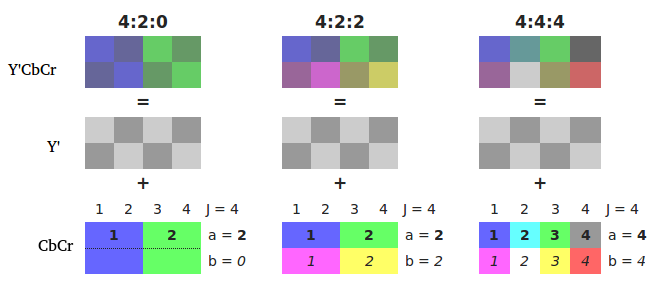
\includegraphics[scale=0.5]{./Figures/png/subamostragem.png}
\caption{Formatos mais comuns de subamostragem da crominância.}
\label{fig:subamostragem}
\end{center}
\end{figure}


%\thispagestyle{fancy}


%\chapter{Considerações finais}
%\thispagestyle{fancy}
%%Capitulo 5 - Considerações finais%

\thispagestyle{fancy}

\section{Conclusões}

Neste trabalho foi apresentado um estudo de compressão de imagens e vídeos, através da análise teórica e implementações simplificadas dos codecs JPEG e MPEG-1. O aspecto perceptual dos vídeos decodificados também foi levado em consideração através da análise do método de quantização inter-adaptativa.

Apesar de necessário, o processo de compressão de informações visuais é responsável pelo surgimento de artefatos nas mesmas. Portanto, o desafio é encontrar um meio termo entre taxa de compressão e qualidade perceptual.

Através da análise desenvolvida neste trabalho pode-se concluir que a utilização do método de quantização inter-adaptativa gera resultados vantajosos para vídeos com alta atividade temporal, enquanto apresenta resultados similares ao codec padrão quando submetido a vídeos com baixa atividade temporal. Dessa forma, os resultados da avaliação objetiva obtidos neste trabalho então condizentes com os resultados subjetivos apresentados em \cite{Li_humanvisual}.

Portanto, a utilização do método de quantização inter-adaptativa é, se não vantajosa, no mínimo equivalente ao padrão H.261.

O mesmo não pode ser dito quando comparamos o codec H.261 utilizando apenas a tabela de quantização ponderada em relação aos codificadores analisados na primeira fase do experimento. Apesar da utilização de uma tabela plana para a quantização dos macroblocos inter codificados possuir embasamento teórico, \cite{ghanbari2003standard}, os resultados obtidos utilizando apenas a tabela ponderada foram os melhores alcançados neste trabalho, divergindo da literatura. No entanto, este resultado requer investigação mais ampla.

\section{Trabalhos futuros}

A próxima fase desta pesquisa tem como objetivos: obter o entendimento a respeito do funcionamento  de codecs mais atuais, como H.262, H.263, H.264 e H.265, de forma a entender as melhorias que foram ascrescentadas gradativamente; analisar de maneira mais profunda os resultados alcançados na segunda fase experimental e estudar outros métodos de melhoria de qualidade perceptual para armazenamento e vídeo conferência.

 % Trocar o nome default Bibliografia para Referências Bibliogrficas



\renewcommand\bibname{Referências Bibliográficas}
%\bibliographystyle{abnt} % Estilo para gerar referncias em conformidade com
                          % as normas brasileiras

%\bibliographystyle{./IEEEtran}
\bibliography{ufpa_tcc_caio}
\clearpage
%\addcontentsline{toc}{chapter}{Referências Bibliográficas}
\addcontentsline{toc}{chapter}{Referências Bibliográficas}
%\bibliography{../public/speech_sa}




%\begin{thebibliography}{999}

%\bibitem{1} \textbf{L.R. Rabiner and R.W. Schafer}, \textit{Digital Processing of Speech Signals}, Prentice-Hall, Inc., Englewood Cliffs, NJ, 1978.
%
%\bibitem{2} \textbf{CUNHA, Celso; CINTRA, Lindley}. \textit{Nova Gramática do Português Moderno}. Edies Joo S da Costa: Lisboa, 2000.
%\end{thebibliography}

\clearpage 
%\addcontentsline{toc}{section}{Apendice:1}
%\appendix
%\chapter{Tabelas de referência em um corpo %GF($2^4$)}
%\thispagestyle{fancy}
%%Tabela de resultados de adições em um corpo GF($2^4$)

\thispagestyle{fancy}
\renewcommand{\thesubsection}{\Alph{section}}
\section{Tabelas de codificação para compressão JPEG}
\label{ap_JPEG}

Objetivando otimizar o processo de compressão JPEG, tabelas Huffman pré definidas são utilizadas para a codificação de entropia. Neste apêndice explica-se como utilizar estas tabelas.

Considerando que se deseja codificar um bloco transformado e quantizado,
\begin{minipage}{1.\textwidth}
\centering
[-26 -3 1 -3 -2 -6 2 -4 1 -4 1 1 5 0 2 0 0 -1 2 0 0 0 0 0 -1 -1 EOB]
\end{minipage}
devemos separar este processo em duas partes:
\begin{enumerate}
\item Codificação do coeficiente DC: supondo que o coeficiente DC do macrobloco imediatamente anterior é $ (-17) $, \footnote{Se for o primeiro macrobloco de uma linha utila-se o valor 0.} tem-se que, segundo a tabela \ref{Cat-coef-JPEG}, a diferença $ d = [-26-(-17)] $ ou $ d=-9 $ pertence à categoria $ k=4 $. Conforme a tabela \ref{Cod-DC}, o código base utilizado para a categoria 4 é 101 e seu tamanho total é de 7 bits, em que os $ k $ bits restantes devem ser os $ k $ bits menos significativos da diferença positiva $ d $ ou os $ k $ bits menos significativos da diferença negativa $ d $ menos $1$. Para a diferença $ d = -9$ os $k$ bits menos significativos são (0111)-1 ou 0110. Logo, a palavra código para o coeficiente DC em questão é 1010110.

\item Codificação do coeficiente AC: sua diferença em relação a codificação de coeficientes DC é que ela leva em consideração o número de zeros que antecedem os coeficientes AC não nulos. Logo o primeiro coeficiente AC não nulo $(-3)$ é codificado como 0100, pois segundo a tabela \ref{Cat-coef-JPEG} ele pertence à categoria 2 sem zeros antecedentes, dando origem ao código base 01, e os dois bits restantes são obtidos de maneira similar a utilizada na codificação de coeficientes DC. 
\end{enumerate}

\begin{table}[!ht]
\centering
\begin{tabular}{|c|c|c|}
\hline
Faixa                                                      & \begin{tabular}[c]{@{}c@{}}Categoria da\\ diferença DC\end{tabular} & \begin{tabular}[c]{@{}c@{}}Categoria\\ AC\end{tabular} \\ \hline
0                                                          & 0                                                                   & N/A                                                    \\ \hline
-1, 1                                                      & 1                                                                   & 1                                                      \\ \hline
-3, -2, 2, 3                                               & 2                                                                   & 2                                                      \\ \hline
-7,..., -4, 4,..., 7                                       & 3                                                                   & 3                                                      \\ \hline
-15,..., -8, 8,..., 15                                     & 4                                                                   & 4                                                      \\ \hline
-31,..., -16, 16,..., 31                                   & 5                                                                   & 5                                                      \\ \hline
-63,..., -32, 32,..., 63                                   & 6                                                                   & 6                                                      \\ \hline
-127,..., -64, 64,..., 127                                 & 7                                                                   & 7                                                      \\ \hline
-255,..., -128, 128,..., 255                               & 8                                                                   & 8                                                      \\ \hline
-511,..., -256, 256,..., 511                               & 9                                                                   & 9                                                      \\ \hline
-1023,..., -512, 5012,..., 1023                            & A                                                                   & A                                                      \\ \hline
-2047,..., -1024, 1024,..., 2047                           & B                                                                   & B                                                      \\ \hline
-4095,..., -2048, 2048,..., 4095                           & C                                                                   & C                                                      \\ \hline
-8191,..., -4096, 4096,..., 8191                           & D                                                                   & D                                                      \\ \hline
-16383,..., -8192, 8192,..., 16383                         & E                                                                   & E                                                      \\ \hline
\multicolumn{1}{|l|}{-32767,..., -16384, 16384,..., 32767} & F                                                                   & N/A                                                    \\ \hline
\end{tabular}
\caption{Categorias de coeficientes de codificação JPEG.}
\label{Cat-coef-JPEG}
\end{table}

\begin{table}[]
\centering
\begin{tabular}{|c|c|c|c|c|c|}
\hline
Categoria & \begin{tabular}[c]{@{}c@{}}Código\\ Base\end{tabular} & Tamanho & Categoria & \begin{tabular}[c]{@{}c@{}}Código \\ Base\end{tabular} & Tamanho \\ \hline
0         & 010                                                   & 3       & 6         & 1110                                                   & 10      \\ \hline
1         & 011                                                   & 4       & 7         & 11110                                                  & 12      \\ \hline
2         & 100                                                   & 5       & 8         & 111110                                                 & 14      \\ \hline
3         & 00                                                    & 5       & 9         & 1111110                                                & 16      \\ \hline
4         & 101                                                   & 7       & A         & 11111110                                               & 18      \\ \hline
5         & 110                                                   & 8       & B         & 111111110                                              & 20      \\ \hline
\end{tabular}
\caption{Códigos JPEG DC.}
\label{Cod-DC}
\end{table}

\begin{table}[!ht]
\centering
\begin{tabular}{|c|c|c|c|c|c|}
\hline
\begin{tabular}[c]{@{}c@{}}Zeros/\\ Categoria\end{tabular} & Código  base     & Tamanho & \begin{tabular}[c]{@{}c@{}}Zeros/\\ Categoria\end{tabular} & Código base      & Tamanho \\ \hline
0/0                                                        & 1010             & 4       & 8/1                                                        & 111111000        & 9       \\ \hline
0/1                                                        & 00               & 2       & 8/2                                                        & 111111111000000  & 15      \\ \hline
0/2                                                        & 01               & 2       & 8/3                                                        & 1111111110110110 & 16      \\ \hline
0/3                                                        & 100              & 3       & 8/4                                                        & 1111111110110111 & 16      \\ \hline
0/4                                                        & 1011             & 4       & 8/5                                                        & 1111111110111000 & 16      \\ \hline
0/5                                                        & 11010            & 5       & 8/6                                                        & 1111111110111001 & 16      \\ \hline
0/6                                                        & 1111000          & 7       & 8/7                                                        & 1111111110111010 & 16      \\ \hline
0/7                                                        & 11111000         & 8       & 8/8                                                        & 1111111110111011 & 16      \\ \hline
0/8                                                        & 1111110110       & 10      & 8/9                                                        & 1111111110111100 & 16      \\ \hline
0/9                                                        & 1111111110000010 & 16      & 8/A                                                        & 1111111110111101 & 16      \\ \hline
0/A                                                        & 1111111110000011 & 16      & 9/1                                                        & 111111001        & 9       \\ \hline
1/1                                                        & 1100             & 4       & 9/2                                                        & 1111111110111110 & 16      \\ \hline
1/2                                                        & 11011            & 5       & 9/3                                                        & 1111111110111111 & 16      \\ \hline
1/3                                                        & 1111001          & 7       & 9/4                                                        & 1111111111000000 & 16      \\ \hline
1/4                                                        & 111110110        & 9       & 9/5                                                        & 1111111111000001 & 16      \\ \hline
1/5                                                        & 11111110110      & 11      & 9/6                                                        & 1111111111000010 & 16      \\ \hline
1/6                                                        & 1111111110000100 & 16      & 9/7                                                        & 1111111111000011 & 16      \\ \hline
1/7                                                        & 1111111110000101 & 16      & 9/8                                                        & 1111111111000100 & 16      \\ \hline
1/8                                                        & 1111111110000110 & 16      & 9/9                                                        & 1111111111000101 & 16      \\ \hline
1/9                                                        & 1111111110000111 & 16      & 9/A                                                        & 1111111111000110 & 16      \\ \hline
1/A                                                        & 1111111110001000 & 16      & A/1                                                        & 111111010        & 9       \\ \hline
2/1                                                        & 11100            & 5       & A/2                                                        & 1111111111000111 & 16      \\ \hline
2/2                                                        & 11111001         & 8       & A/3                                                        & 1111111111001000 & 16      \\ \hline
2/3                                                        & 1111110111       & 10      & A/4                                                        & 1111111111001001 & 16      \\ \hline
2/4                                                        & 111111110100     & 12      & A/5                                                        & 1111111111001010 & 16      \\ \hline
2/5                                                        & 1111111110001001 & 16      & A/6                                                        & 1111111111001011 & 16      \\ \hline
2/6                                                        & 1111111110001010 & 16      & A/7                                                        & 1111111111001100 & 16      \\ \hline
2/7                                                        & 1111111110001011 & 16      & A/8                                                        & 1111111111001101 & 16      \\ \hline
\end{tabular}
\caption{Códigos JPEG AC.}
\label{Cod-AC1}
\end{table}


\begin{table}[!ht]
\centering
\begin{tabular}{|c|c|c|c|c|c|}
\hline
\begin{tabular}[c]{@{}c@{}}Zeros/\\ Categoria\end{tabular} & Código  base     & Tamanho & \begin{tabular}[c]{@{}c@{}}Zeros/\\ Categoria\end{tabular} & Código base      & Tamanho \\ \hline
2/8                                                        & 1111111110001100 & 16      & A/9                                                        & 1111111111001110 & 16      \\ \hline
2/9                                                        & 1111111110001101 & 16      & A/A                                                        & 1111111111001111 & 16      \\ \hline
2/A                                                        & 1111111110001110 & 16      & B/1                                                        & 1111111001       & 10      \\ \hline
3/1                                                        & 111010           & 6       & B/2                                                        & 1111111111010000 & 16      \\ \hline
3/2                                                        & 111110111        & 9       & B/3                                                        & 1111111111010001 & 16      \\ \hline
3/3                                                        & 111111110101     & 12      & B/4                                                        & 1111111111010010 & 16      \\ \hline
3/4                                                        & 1111111110001111 & 16      & B/5                                                        & 1111111111010011 & 16      \\ \hline
3/5                                                        & 1111111110010000 & 16      & B/6                                                        & 1111111111010100 & 16      \\ \hline
3/6                                                        & 1111111110010001 & 16      & B/7                                                        & 1111111111010101 & 16      \\ \hline
3/7                                                        & 1111111110010010 & 16      & B/8                                                        & 1111111111010110 & 16      \\ \hline
3/8                                                        & 1111111110010011 & 16      & B/9                                                        & 1111111111010111 & 16      \\ \hline
3/9                                                        & 1111111110010100 & 16      & B/A                                                        & 1111111111011000 & 16      \\ \hline
3/A                                                        & 1111111110010101 & 16      & C/1                                                        & 1111111010       & 10      \\ \hline
4/1                                                        & 111011           & 6       & C/2                                                        & 1111111111011001 & 16      \\ \hline
4/2                                                        & 1111111000       & 10      & C/3                                                        & 1111111111011010 & 16      \\ \hline
4/3                                                        & 1111111110010110 & 16      & C/4                                                        & 1111111111011011 & 16      \\ \hline
4/4                                                        & 1111111110010111 & 16      & C/5                                                        & 1111111111011100 & 16      \\ \hline
4/5                                                        & 1111111110011000 & 16      & C/6                                                        & 1111111111011101 & 16      \\ \hline
4/6                                                        & 1111111110011001 & 16      & C/7                                                        & 1111111111011110 & 16      \\ \hline
4/7                                                        & 1111111110011010 & 16      & C/8                                                        & 1111111111011111 & 16      \\ \hline
4/8                                                        & 1111111110011011 & 16      & C/9                                                        & 1111111111100000 & 16      \\ \hline
4/9                                                        & 1111111110011100 & 16      & C/A                                                        & 1111111111100001 & 16      \\ \hline
4/A                                                        & 1111111110011101 & 16      & D/1                                                        & 11111111000      & 10      \\ \hline
5/1                                                        & 1111010          & 7       & D/2                                                        & 1111111111100010 & 16      \\ \hline
5/2                                                        & 11111110111      & 11      & D/3                                                        & 1111111111100011 & 16      \\ \hline
5/3                                                        & 1111111110011110 & 16      & D/4                                                        & 1111111111100100 & 16      \\ \hline
5/4                                                        & 1111111110011111 & 16      & D/5                                                        & 1111111111100101 & 16      \\ \hline
5/5                                                        & 1111111110100000 & 16      & D/6                                                        & 1111111111100110 & 16      \\ \hline
5/6                                                        & 1111111110100001 & 16      & D/7                                                        & 1111111111100111 & 16      \\ \hline
\end{tabular}
\caption{Códigos JPEG AC (continuação.)}
\label{Cod-AC2}
\end{table}

\begin{table}[!ht]
\centering
\begin{tabular}{|c|c|c|c|c|c|}
\hline
\begin{tabular}[c]{@{}c@{}}Zeros/\\ Categoria\end{tabular} & Código  base     & Tamanho & \begin{tabular}[c]{@{}c@{}}Zeros/\\ Categoria\end{tabular} & Código base      & Tamanho \\ \hline
5/7                                                        & 1111111110100010 & 16      & D/8                                                        & 1111111111101000 & 16      \\ \hline
5/8                                                        & 1111111110100011 & 16      & D/9                                                        & 1111111111101001 & 16      \\ \hline
5/9                                                        & 1111111110100100 & 16      & D/A                                                        & 1111111111101010 & 16      \\ \hline
5/A                                                        & 1111111110100101 & 16      & E/1                                                        & 1111111111101011 & 11      \\ \hline
6/1                                                        & 1111011          & 7       & E/2                                                        & 1111111111101100 & 16      \\ \hline
6/2                                                        & 111111110110     & 12      & E/3                                                        & 1111111111101101 & 16      \\ \hline
6/3                                                        & 1111111110100110 & 16      & E/4                                                        & 1111111111101110 & 16      \\ \hline
6/4                                                        & 1111111110100111 & 16      & E/5                                                        & 1111111111101111 & 16      \\ \hline
6/5                                                        & 1111111110101000 & 16      & E/6                                                        & 1111111111110000 & 16      \\ \hline
6/6                                                        & 1111111110101001 & 16      & E/7                                                        & 1111111111110001 & 16      \\ \hline
6/7                                                        & 1111111110101010 & 16      & E/8                                                        & 1111111111110010 & 16      \\ \hline
6/8                                                        & 1111111110101011 & 16      & E/9                                                        & 1111111111110011 & 16      \\ \hline
6/9                                                        & 1111111110101100 & 16      & E/A                                                        & 1111111111110100 & 16      \\ \hline
6/A                                                        & 1111111110101101 & 16      & F/0                                                        & 11111111001      & 11      \\ \hline
7/1                                                        & 11111010         & 8       & F/1                                                        & 1111111111110101 & 16      \\ \hline
7/2                                                        & 111111110111     & 12      & F/2                                                        & 1111111111110110 & 16      \\ \hline
7/3                                                        & 1111111110101110 & 16      & F/3                                                        & 1111111111110111 & 16      \\ \hline
7/4                                                        & 1111111110101111 & 16      & F/4                                                        & 1111111111111000 & 16      \\ \hline
7/5                                                        & 1111111110110000 & 16      & F/5                                                        & 1111111111111001 & 16      \\ \hline
7/6                                                        & 1111111110110001 & 16      & F/6                                                        & 1111111111111010 & 16      \\ \hline
7/7                                                        & 1111111110110010 & 16      & F/7                                                        & 1111111111111011 & 16      \\ \hline
7/8                                                        & 1111111110110011 & 16      & F/8                                                        & 1111111111111100 & 16      \\ \hline
7/9                                                        & 1111111110110100 & 16      & F/9                                                        & 1111111111111101 & 16      \\ \hline
7/A                                                        & 1111111110110101 & 16      & F/A                                                        & 1111111111111110 & 16      \\ \hline
\end{tabular}
\caption{Códigos JPEG AC (continuação).}
\label{Cod-AC3}
\end{table}
%  \clearpage \addcontentsline{toc}{section}{Apêndice 2:}

%% -- aqui termina o TCC
\end{document}
